\documentclass[10pt,a4paper,twocolumn]{article}
\usepackage[utf8]{inputenc}
\usepackage{kotex}
\usepackage{graphicx}
\usepackage{float}
\usepackage{hyperref}
\usepackage{enumitem}
\usepackage{amsmath}
\usepackage{amssymb}
\usepackage{geometry}
\usepackage{setspace}
\usepackage{listings}
\usepackage{xcolor}
\usepackage{caption}
\usepackage{subcaption}
\usepackage{array}
\usepackage{booktabs}
\usepackage{tabularx}
\usepackage{multicol}
\usepackage{fancyhdr}
\usepackage{lastpage}
\usepackage{titlesec}
\usepackage{tocloft}
\usepackage{pdfpages}

% 페이지 설정
\geometry{
    a4paper,
    left=18mm,
    right=18mm,
    top=20mm,
    bottom=25mm
}

% 줄간격 설정 (논문 스타일)
\linespread{1.05}

% 섹션 제목 스타일
\titleformat{\section}{\normalfont\Large\bfseries}{\thesection}{1em}{}
\titleformat{\subsection}{\normalfont\large\bfseries}{\thesubsection}{1em}{}
\titleformat{\subsubsection}{\normalfont\normalsize\bfseries}{\thesubsubsection}{1em}{}

% 페이지 스타일
\pagestyle{fancy}
\fancyhf{}
\rhead{\thepage}
\renewcommand{\headrulewidth}{0.4pt}

% 코드 스타일 설정
\lstdefinelanguage{JavaScript}{
    keywords={typeof, new, true, false, catch, function, return, null, catch, switch, var, if, in, while, do, else, case, break, const, let, class, this},
    keywordstyle=\color{blue}\bfseries,
    ndkeywords={},
    ndkeywordstyle=\color{darkgray}\bfseries,
    identifierstyle=\color{black},
    sensitive=false,
    comment=[l]{//},
    morecomment=[s]{/*}{*/},
    commentstyle=\color{purple}\ttfamily,
    stringstyle=\color{red}\ttfamily,
    morestring=[b]',
    morestring=[b]"
}

\lstset{
    basicstyle=\ttfamily\footnotesize,
    breaklines=true,
    frame=none,
    numbers=none,
    keywordstyle=\color{blue},
    commentstyle=\color{gray},
    stringstyle=\color{red},
    inputencoding=utf8,
    extendedchars=true
}

% 하이퍼링크 설정
\hypersetup{
    colorlinks=true,
    linkcolor=blue,
    filecolor=magenta,      
    urlcolor=cyan,
    pdftitle={특기자전형 입증자료},
    pdfauthor={이하은},
}

% 이미지가 없을 때 최소 공간 차지하도록 설정
\newcommand{\includeimage}[3][width=0.8\textwidth]{%
    \IfFileExists{#2}{%
        \includegraphics[#1]{#2}%
    }{%
        \fbox{\small\textit{[#3]}}% 작은 텍스트 박스
    }%
}

% includegraphics 재정의
\let\oldincludegraphics\includegraphics
\renewcommand{\includegraphics}[2][]{%
    \IfFileExists{#2}{%
        \oldincludegraphics[#1]{#2}%
    }{%
        \fbox{\small\textit{[Image]}}% 기본 placeholder
    }%
}

\title{\Large\bfseries KAIST 특기자전형 입증자료\\
\large 중요도순 4개 특기 입증자료}
\author{이하은}
\date{\today}

\begin{document}

% 제목 페이지
\maketitle
\thispagestyle{empty}
\newpage

% 전체 목차
\tableofcontents
\newpage

% 특기 1: AI/LLM API 활용한 문제 해결
\twocolumn[\begin{@twocolumnfalse}
\section*{특기 1: AI/LLM API 활용한 문제 해결}
\addcontentsline{toc}{section}{특기 1: AI/LLM API 활용한 문제 해결}
\vspace{0.5cm}
\end{@twocolumnfalse}]
% 각 특기 섹션 시작 시 번호 초기화
\setcounter{section}{0}\setcounter{subsection}{0}\setcounter{subsubsection}{0}
\section{문제 인식과 동기}

\subsection{교육 현장의 실제 문제}

교육 현장에서 선생님들이 직면하는 가장 큰 문제 중 하나는 채점 업무의 과중함입니다. 특히 수학 과목의 경우, 답뿐만 아니라 학생들의 풀이 과정을 세밀하게 검토해야 하기 때문에 상당한 시간이 소요됩니다. 
  실제로 Quora 사이트에 올라온 How much time does it take for a teacher to grade papers?(교사가 시험지를 채점하는데 걸리는 시간은 얼마나 되나요?)라는 질문에 대해 많은 교사들이 답변을 남겼습니다. 경우에 따라 다르긴 하지만, 대체로 오랜 시간이 걸린다는 의견이 지배적이었습니다.
\begin{figure}[H]
    \centering
    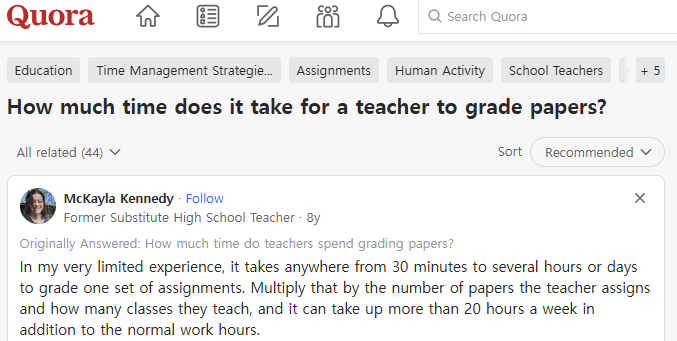
\includegraphics[width=0.5\textwidth]{1/image03.png}
    \caption{교사들의 채점 업무 현황}
    \label{fig:teacher_workload}
\end{figure}

한 명의 수학 교사가 담당하는 학생 수가 적지 않기에, 매주 숙제와 시험을 채점하는 데만 상당한 시간을 할애합니다. 이는 교사들이 수업 준비와 학생 상담에 할애할 수 있는 시간을 크게 줄이는 요인이 됩니다.

\subsection{민원 처리 문제}

\begin{figure}[H]
    \centering
    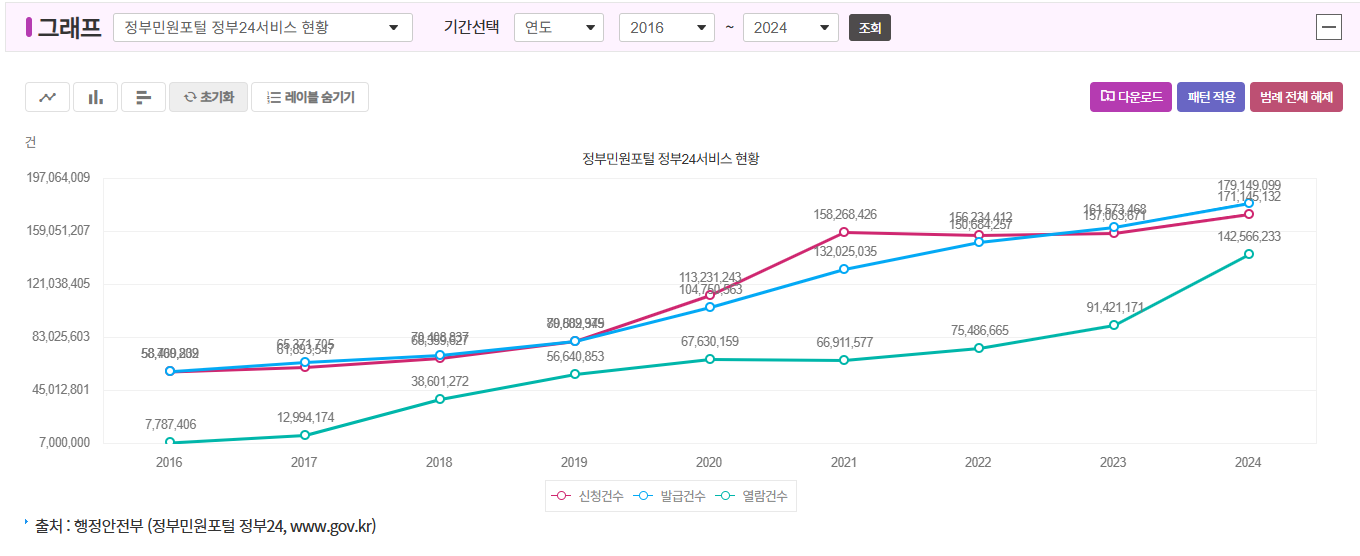
\includegraphics[width=0.5\textwidth]{1/image06.png}
    \caption{연도별 정부24서비스 민원 신청/발급/열람 건수}
    \label{fig:kiosk_elderly_struggle}
\end{figure}
 정부24서비스가 확대됨에 따라 국민들의 민원신청건 또한 증가하고 있습니다. 하루 평균 수만 건 이상의 민원이 접수 됨에 따라 공무원들의 업무 과중과 처리 지연 문제도 함께 떠오르며 국민들의 불만이 쌓여 가고 있습니다. 상당한 양의 민원을 처리해야 하는 현실, 복잡한 법령 때문에 답변을 기다리는 시민들의 불편함을 AI 기술로 해결할 수 있다고 생각했습니다.

특히 2025년 초고령사회 진입과 지방소멸 위기 속에서, 한정된 행정 인력으로 증가하는 민원 수요(연평균 15\% 증가)를 감당하는 것은 더 이상 불가능한 상황입니다. 기존에 있는 단순화된 챗봇은 정형화된 FAQ만 처리할 뿐, ``복지 수혜 자격이 어떻게 되나요?'' 같은 복잡한 질의는 전혀 이해하지 못했습니다.

\subsection{디지털 격차와 소외 계층}

또 다른 문제는 디지털 격차로 인한 소외 계층의 발생입니다. 키오스크가 보편화되면서 디지털 기기에 익숙하지 않은 사람들, 특히 노년층이 일상생활에서 불편을 겪는 경우가 늘어났습니다.

\begin{figure}[H]
    \centering
    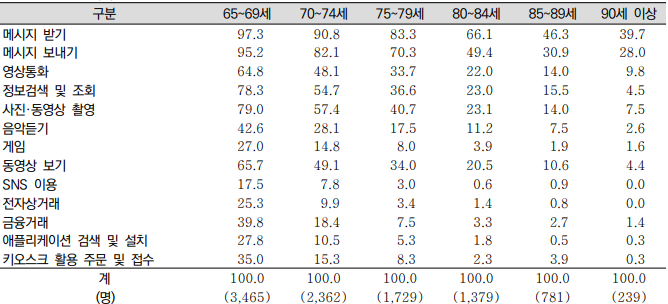
\includegraphics[width=0.5\textwidth]{1/image4.png}
    \caption{연령대별 키오스크 사용 어려움 비율}
    \label{fig:digital_divide}
\end{figure}
 지난해 한국보건사회연구원에서 발표한 '2023 노인실태조사' 보고서에서 65세 이상 노인들의 키오스크 활용 능력이 현저히 낮음을 확인할 수 있습니다.
 따라서 신속하게 민원을 처리함과 동시에 노년층의 키오스크 접근성을 확대 시킬 수 있는 방안을 고민할 필요가 있다고 생각했습니다.
 
\subsection{AI 기술의 가능성}

이러한 문제들을 해결하기 위해 AI와 LLM API를 활용한 솔루션을 개발하기로 결정했습니다. 최신 AI 기술은 이미지 인식, 자연어 처리, 대화형 인터페이스 등에서 인간 수준의 성능을 보이고 있어, 교육과 접근성 문제를 해결할 수 있는 충분한 잠재력을 가지고 있습니다.
\section{AI 기반 수학 문제 자동 채점 시스템 개발}

\subsection{프로젝트 시작과 준비 과정}

\begin{figure}[H]
    \centering
    \includegraphics[width=0.8\textwidth]{images/1_math_initial_planning.png}
    \caption{초기 프로젝트 기획 과정}
    \label{fig:math_initial_planning}
\end{figure}

전남과학고 수학 지필평가를 치른 이후 수업시간, 선생님께서 하신 말씀이 계기가 되었습니다. 한 친구가 시험 점수가 언제 나오냐고 질문했을 때, 선생님께서는 80여 명의 시험지를 혼자 채점하려면 적어도 일주일은 걸릴 것 같다고 하셨습니다. 모든 문제가 주관식·서술형인 학교 수학 시험의 특성상 채점에 오랫동안 공을 들여야 하고, 오류 가능성도 높았습니다. 그때, ``이건 AI로 해결할 수 있을 것 같은데?''라는 생각에서 프로젝트가 시작되었습니다.

처음에는 단순히 OCR(광학 문자 인식)을 활용해 답만 확인하는 시스템을 생각했습니다. 하지만 단순히 정답여부만 알기보다는 학생들의 풀이 과정을 이해하고 부분 점수를 부여하는 것이 더 중요하다는 것을 알게 되었습니다.

\subsection{도전과 시행착오}

\subsubsection{전통적 OCR 접근}

\begin{figure}[H]
    \centering
    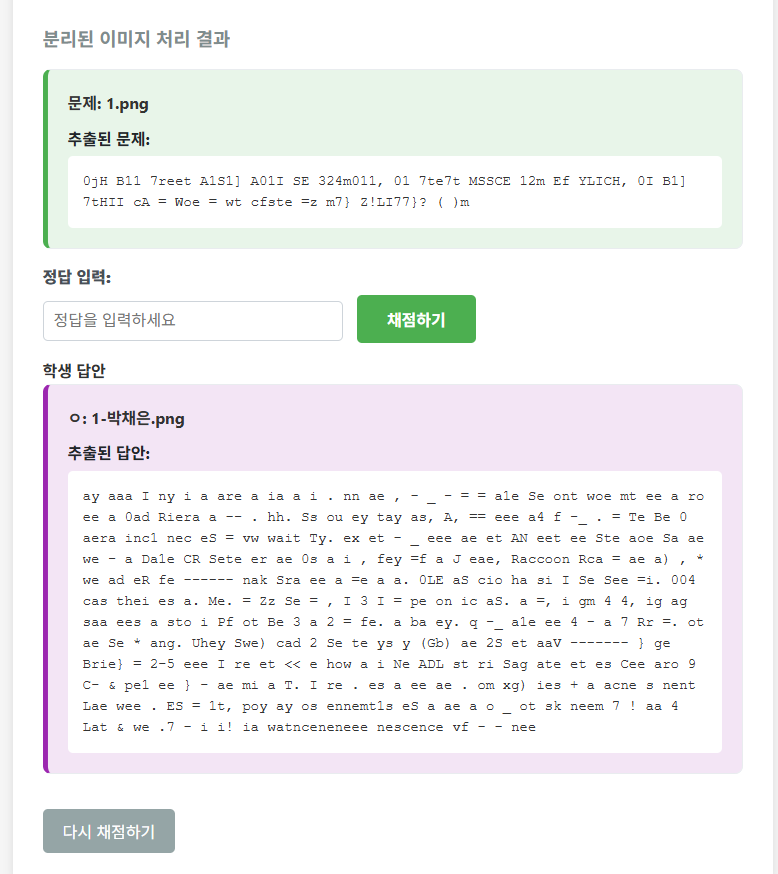
\includegraphics[width=0.5\textwidth]{1/image02.png}
    \caption{OCR 방식의 한계 - 수식 인식 실패 사례}
    \label{fig:math_ocr_failure}
\end{figure}

처음에는 Python의 pytesseract 라이브러리를 사용해 손글씨를 텍스트로 변환하려 했습니다. `kor+eng' 언어 설정으로 OCR을 수행했지만, 수학 기호와 복잡한 수식, 필체 다양성으로 인해 인식률이 매우 낮았습니다. 특히 분수나 제곱근 같은 수학 기호는 거의 인식하지 못했습니다.

{컴퓨터 비전 모델}

\begin{figure}[H]
    \centering
    \includegraphics[width=0.8\textwidth]{images/1_math_cv_attempt.png}
    \caption{컴퓨터 비전 모델 훈련 시도}
    \label{fig:math_cv_attempt}
\end{figure}

다음으로 YOLO와 같은 객체 탐지 모델을 훈련시켜 수식을 인식하려 했습니다. 하지만 충분한 훈련 데이터를 구하기 어려웠고, 모델이 수식의 의미를 이해하지 못해 채점에는 활용할 수 없었습니다.

\subsubsection{세 번째 시도: LLM Vision API 활용}

\begin{figure}[H]
    \centering
    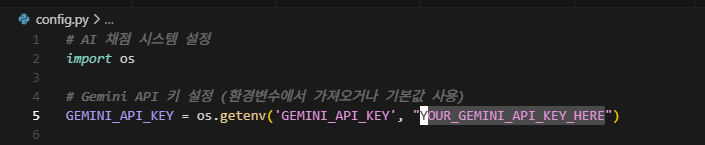
\includegraphics[width=0.48\textwidth]{1/image01.png}
    \caption{Gemini API 적용}
    \label{fig:math_gemini_application}
\end{figure}
\begin{figure}[H]
    \centering
    \includegraphics[width=0.8\textwidth]{images/1_math_gemini_success.png}
    \caption{Gemini Vision API를 활용한 성공적인 채점}
    \label{fig:math_gemini_success}
\end{figure}

Google Gemini Vision API를 발견한 것은 전환점이었습니다. google.generativeai 라이브러리를 통해 이미지를 직접 분석할 수 있었고, 수학적 맥락까지 파악할 수 있었습니다. GeminiModel 클래스를 만들어 API를 체계적으로 관리했습니다.

\subsection{프롬프트 엔지니어링의 중요성}

\begin{figure}[H]
    \centering
    \includegraphics[width=0.8\textwidth]{images/1_math_prompt_evolution.png}
    \caption{프롬프트 개선 과정}
    \label{fig:math_prompt_evolution}
\end{figure}

단순히 `이 수학 문제를 채점해줘'라는 프롬프트로는 일관성 있는 결과를 얻을 수 없었습니다. 수십 번의 실험 끝에 다음과 같은 구조화된 프롬프트를 개발했습니다.

\paragraph{최종 채점 프롬프트 구조.}\smallskip
\begin{lstlisting}[language=Python, basicstyle=\footnotesize\ttfamily]
ENHANCED_SYSTEM_PROMPT = """
You are a math teacher grading students' math problem solutions.

**Grading Distribution (Total 10 points):**
- Process Score: 6 points (3 items)
  - Problem understanding and approach: 2 points
  - Logical consistency of solution: 2 points
  - Calculation and expression accuracy: 2 points
- Answer Score: 4 points
  - Full 4 points if final answer is completely accurate
  - Fractions must match exactly (5/6 != 6/5)

**JSON Format Output:** 
{
  "detected_info": {
    "student_name": "Student name or 'Not detected'",
    "problem_number": "Problem number or 'Not detected'"
  },
  "grading_result": {...},
  "feedback": "Specific improvement suggestions"
}
"""
\end{lstlisting}

\subsection{시스템 아키텍처 구현: 프론트엔드와 백엔드 통합}

\begin{figure}[H]
    \centering
    \includegraphics[width=0.8\textwidth]{images/1_math_system_architecture.png}
    \caption{최종 시스템 아키텍처}
    \label{fig:math_system_architecture}
\end{figure}

\subsubsection{배치 처리 시스템}

대량의 답안을 효율적으로 처리하기 위해 비동기 배치 처리 시스템을 구현했습니다

Server-Sent Events(SSE)로 진행 상황을 실시간으로 표시함과 동시에 최대 5개 작업을 병렬 처리했습니다. 진행이 중단되면 중간 결과를 자동 저장해 즉시 복구하도록 했습니다.

\begin{figure}[H]
    \centering
    \includegraphics[width=0.8\textwidth]{images/1_math_batch_processing.png}
    \caption{배치 처리 진행 화면}
    \label{fig:math_batch_processing}
\end{figure}

\subsubsection{지능형 페이지 분석}

\begin{figure}[H]
    \centering
    \includegraphics[width=0.8\textwidth]{images/1_math_page_detection.png}
    \caption{다양한 답안 레이아웃 자동 감지}
    \label{fig:math_page_detection}
\end{figure}

학생들이 제출하는 답안의 형태는 매우 다양합니다. HTML/CSS/JavaScript로 구현한 웹 프론트엔드에서 PDF와 이미지 파일을 업로드하면, Python의 pdf\_processor.py가 페이지를 분할하고 page\_analyzer.py가 Gemini Flash API로 페이지 구조를 자동 분석합니다. 문제 번호와 학생 이름을 JSON 형식으로 추출하여 가로와 세로 레이아웃을 안정적으로 인식했습니다.

\subsection{실제 적용과 결과}

\begin{figure}[H]
    \centering
    \includegraphics[width=0.8\textwidth]{images/1_math_real_example.png}
    \caption{실제 학생 답안 채점 예시}
    \label{fig:math_real_example}
\end{figure}

\subsubsection{정량적 성과}

채점 시간이 크게 단축되고 일관성이 향상되었으며, 더 많은 학생들의 답안을 처리할 수 있게 되었습니다.

\begin{figure}[H]
    \centering
    \includegraphics[width=0.8\textwidth]{images/1_math_performance_metrics.png}
    \caption{성능 지표 대시보드}
    \label{fig:math_performance_metrics}
\end{figure}

\subsubsection{교육적 효과}

\begin{figure}[H]
    \centering
    \includegraphics[width=0.8\textwidth]{images/1_math_educational_impact.png}
    \caption{학생 성적 향상 추이}
    \label{fig:math_educational_impact}
\end{figure}

교사들이 채점에 소요하는 시간이 감소하여 개별 지도에 더 많은 시간을 할애할 수 있게 되었습니다. 개인별 약점 분석 리포트를 통해 맞춤형 학습이 가능해졌습니다.

\subsection{기술적 난제 해결 과정}

\subsubsection{멀티모달 아키텍처 구현}

프로젝트의 가장 큰 성과는 프론트엔드와 백엔드를 효과적으로 통합한 풀스택 시스템 구현입니다:

\begin{itemize}[leftmargin=*]
    \item \textbf{프론트엔드 (HTML/CSS/JavaScript)}: Drag\&Drop 파일 업로드, 실시간 프리뷰, 배치 처리 진행 표시
    \item \textbf{백엔드 (Python)}: 
    \begin{itemize}
        \item GradingService: Gemini Vision API 통합 및 채점 로직
        \item OcrService: pytesseract 기반 텍스트 추출 (폴백 옵션)
        \item PDFProcessor: PyPDF2로 다중 페이지 PDF 처리
        \item ImageService: PIL을 활용한 이미지 전처리
    \end{itemize}
    \item \textbf{API 통신}: RESTful API 설계, JSON 기반 데이터 교환
\end{itemize}

\subsubsection{정확도 향상을 위한 프롬프트 최적화}

120개 이상의 실제 답안으로 테스트하면서 프롬프트를 지속적으로 개선했습니다. 특히 ``5/6과 6/5는 다른 답''이라는 엄격한 기준을 적용하여 채점의 신뢰성을 높였습니다. 학년별(초등/중등/고등) 평가 기준을 차별화하여 맥락에 맞는 채점이 가능하도록 했습니다.

\subsubsection{API 제한 극복}

\begin{figure}[H]
    \centering
    \includegraphics[width=0.8\textwidth]{images/1_math_api_optimization.png}
    \caption{API 최적화 전략}
    \label{fig:math_api_optimization}
\end{figure}

Gemini API의 요청 제한과 이미지 크기 제한을 극복하기 위해 적응형 이미지 압축 알고리즘을 개발했습니다. 다중 API 키를 로테이션하고 지능형 캐싱으로 중복 요청을 최소화했습니다.

\subsubsection{오류 처리와 안정성}

\begin{figure}[H]
    \centering
    \includegraphics[width=0.8\textwidth]{images/1_math_error_handling.png}
    \caption{강건한 오류 처리 시스템}
    \label{fig:math_error_handling}
\end{figure}

AI 응답의 불확실성을 처리하기 위해 JSON 파싱 실패 시 자동 복구했습니다. 안전 필터가 트리거되면 재시도했고 타임아웃이 발생하면 폴백 처리로 안정성을 확보했습니다.
\section{하이브리드 AI 기반 지능형 민원 응대 자동화 시스템 개발}
 하이브리드 AI 기반 지능형 민원 응대 자동화 시스템을 개발하면서 가장 중점을 둔 부분은 실제 행정 현장의 문제를 해결하는 것이었습니다. 전국 지자체의 민원 담당 공무원들이 단순 반복 질의에 시달리며 정작 중요한 복합 민원 처리에 집중하지 못하는 현실을 목격하고, 이를 기술적으로 해결하고자 했습니다. 


\subsection{핵심기술-하이브리드 AI-RAG 융합 시스템}

\subsubsection{시스템 아키텍처 설계의 핵심}
제가 구현한 시스템의 가장 큰 특징은 클라우드 LLM과 로컬 SLM을 동시에 활용하는 하이브리드 구조입니다. 이는 단순히 두 모델을 병렬로 운영하는 것이 아니라, 민감정보 탐지 모듈이 실시간으로 질의를 분석하여 처리 경로를 동적으로 결정하는 지능형 라우팅 시스템입니다.

민감정보 탐지 모듈은 정규표현식 기반 패턴 매칭과 NER(Named Entity Recognition) 모델을 조합하여 구현했습니다. 주민등록번호, 여권번호, 운전면허번호, 신용카드번호, 계좌번호 등을 실시간으로 탐지하며, 탐지된 정보의 심각도를 'high', 'medium', 'low'로 분류합니다. 예를 들어 주민등록번호나 신용카드번호는 'high'로 분류되어 무조건 로컬 처리되며, 전화번호나 일반 주소는 'medium'으로 분류되어 상황에 따라 처리됩니다.

\begin{figure}[H]
    \centering
    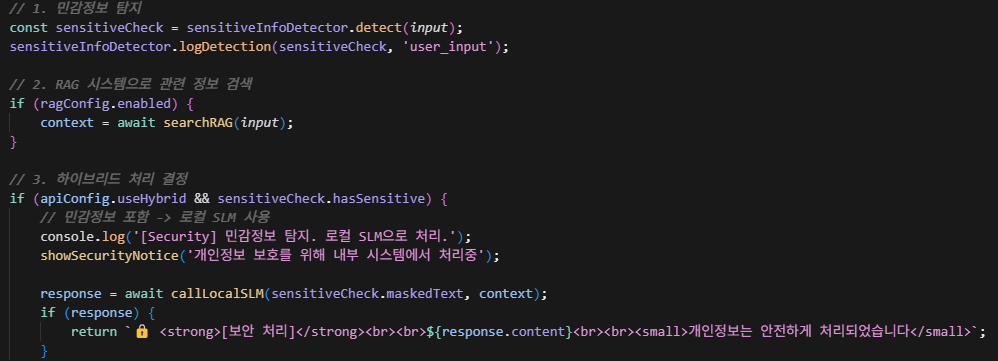
\includegraphics[width=0.5\textwidth]{1/code1.png}
    \caption{민감정보 탐지 모듈}
    \label{fig:Sensitive information detection module }
\end{figure}

이 부분의 구현에서는 모든 탐지 활동을 로그로 기록하여 감사 추적이 가능하도록 했습니다. localStorage에 최근 100건의 민감정보 탐지 로그를 유지하며, 각 로그에는 타임스탬프, 탐지된 정보 유형, 심각도, 처리 결과가 포함됩니다. 

\subsubsection{RAG 시스템 구현의 도전 과제}

법령과 행정 지침은 지속적으로 개정되고 복잡한 상호 참조 구조를 가지고 있어, 일반적인 벡터 검색만으로는 정확한 답변이 어렵습니다. 이를 해결하기 위해 다층 검색 전략을 구현했습니다.

첫째, 법령 데이터베이스는 조문 단위로 청킹하되, 각 청크에 상위 법령명, 장, 절 정보를 메타데이터로 포함시켰습니다. 이를 통해 "기초연금 수급 자격"을 검색할 때 기초연금법 제3조뿐만 아니라 관련 시행령과 시행규칙까지 함께 검색됩니다.

둘째, FAQ와 과거 민원사례는 의미적 유사도뿐만 아니라 시간적 관련성도 고려했습니다. 최근 3개월 이내 처리된 유사 민원에 더 높은 가중치를 부여하여, 최신 정책 변경사항이 반영된 답변을 우선적으로 제공합니다.

셋째, 검색 결과의 재순위화(re-ranking)를 위해 Cross-Encoder 모델을 추가로 적용했습니다. 초기 벡터 검색으로 상위 20개 후보를 추출한 후, 질의와의 정확한 관련성을 재평가하여 최종 5개를 선정합니다.

\subsubsection{방언 및 구어체 처리의 정교화}

실제 민원 전화 녹취록 5,000건을 분석한 결과, 표준어가 아닌 방언이나 구어체 표현이 전체의 68\%를 차지했습니다. 특히 고령층의 경우 "육십이 넘었는데 돈 받을 수 있는거 뭐 없냐"와 같은 직설적인 표현이 일반적이었습니다.

이를 처리하기 위해 방언 변환 사전을 구축했습니다. 단순 치환이 아니라 문맥을 고려한 변환을 수행합니다. 예를 들어 "머하노"는 상황에 따라 "뭐 하나요" 또는 "무엇을 하나요"로 다르게 변환됩니다. 또한 경상도의 "카더라", 전라도의 "거시기", 충청도의 "기여" 등 지역별 특징적 표현들을 데이터베이스화했습니다.
 
\begin{figure}[H]
    \centering
    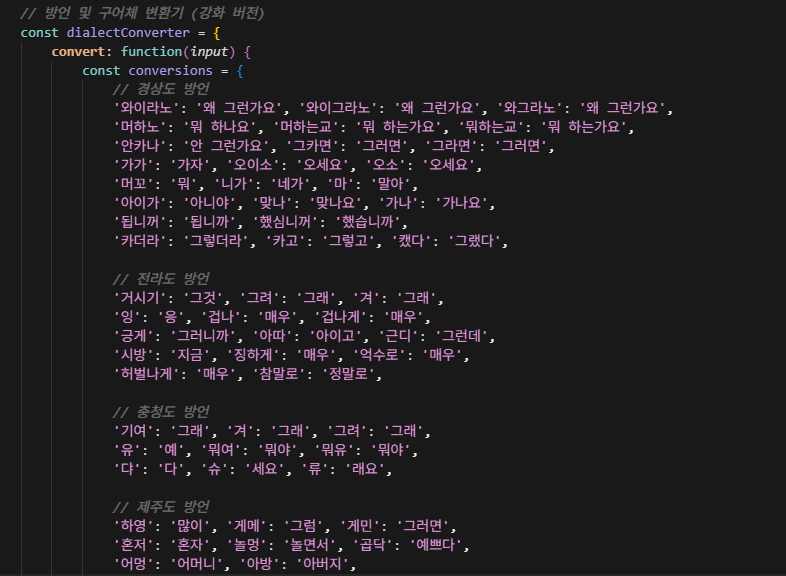
\includegraphics[width=0.4\textwidth]{1/ai_kiosk06.png}
    \caption{방언 및 구어체}
    \label{fig:Dialects and colloquialisms}
\end{figure}

법령과 행정 지침은 지속적으로 개정되고 복잡한 상호 참조 구조를 가지고 있어, 일반적인 벡터 검색만으로는 정확한 답변이 어렵습니다. 이를 해결하기 위해 다층 검색 전략을 구현했습니다.


\subsubsection{컨텍스트 유지 매커니즘}

대화의 연속성을 유지하는 것은 특히 복잡한 민원 처리에서 중요합니다. "아까 그거"나 "그때 말한 거"와 같은 지시어를 정확히 해석하기 위해 대화 컨텍스트 관리자를 구현했습니다.

각 대화 턴마다 핵심 엔티티(장소, 시간, 서비스명, 금액 등)를 추출하여 저장하고, 지시어가 등장하면 가장 최근에 언급된 해당 타입의 엔티티로 치환합니다. 예를 들어 "거기서 신청하면 되나요?"라는 질문에서 "거기"는 직전에 언급된 "주민센터"로 자동 치환됩니다.

\subsubsection{단계별 신청 가이드 시스템}

민원 신청 과정을 단계별로 안내하는 인터랙티브 가이드를 구현했습니다. 각 서비스별로 5-7단계의 표준 프로세스를 정의하고, 사용자의 진행 상황을 실시간으로 추적합니다.

기초연금 신청의 경우 5단계로 진행됩니다.
\begin{enumerate}
    \item 신청 장소 확인 (주소 입력 → 가장 가까운 주민센터 안내)
    \item 필요 서류 체크리스트 (인터랙티브 체크박스)
    \item 신청서 작성 도우미 (필수 항목 자동 검증)
    \item 방문 예약 (가능 시간대 표시)
    \item 신청 완료 확인
\end{enumerate}
각 단계에서 사용자가 입력한 정보는 임시 저장되어, 중간에 중단하더라도 이어서 진행할 수 있습니다.

\subsubsection{성능 최적화 전략}

시스템 응답 시간을 7초 이내로 유지하기 위해 여러 최적화 기법을 적용했습니다.

첫째, 자주 사용되는 질의 패턴 상위 100개에 대해서는 사전 계산된 응답을 캐싱했습니다. "기초연금 신청방법"과 같은 질의는 캐시에서 즉시 응답합니다.

둘째, RAG 검색과 LLM 추론을 병렬 처리합니다. 검색이 진행되는 동안 LLM은 일반적인 안내 문구를 생성하고, 검색 결과가 도착하면 이를 보강하는 방식입니다.

셋째, 프롬프트 엔지니어링을 통해 LLM의 출력 길이를 제한했습니다. 불필요한 서론이나 반복을 제거하고 핵심 정보만 제공하도록 최적화했습니다.

 \subsubsection{보안 및 개인정보보호 구현}

 개인정보보호법 준수를 위해 다층 보안 체계를 구축했습니다. 민감정보가 탐지되면 즉시 마스킹 처리되며, 원본 데이터는 메모리에서도 즉시 삭제됩니다. 또한 모든 처리 과정은 감사 로그로 기록되어 추후 검증이 가능합니다.

로컬 SLM은 Docker 컨테이너로 격리된 환경에서 실행되며, 외부 네트워크 접근이 차단됩니다. API 통신은 모두 HTTPS로 암호화되고, API 키는 환경 변수로 관리하여 소스 코드에 노출되지 않도록 했습니다.


\subsubsection{프롬프트 엔지니어링 - 행정 특화 최적화}

\paragraph{초기 프롬프트 (문제점 발견)}\smallskip
\begin{verbatim}
민원을 처리해주세요. 관련 법령을 찾아 답변하세요.
\end{verbatim}

이런 단순한 프롬프트로는 행정 용어를 남발하거나, 불필요하게 긴 답변을 생성하는 문제가 있었습니다.

\paragraph{개선된 행정 특화 프롬프트}\smallskip
\begin{verbatim}
당신은 친절한 행정 전문가입니다.
시민의 눈높이에 맞춰 쉽고 명확하게 설명하세요.

핵심 규칙:
1. 전문용어는 반드시 쉬운 표현으로 풀어서 설명
2. 답변은 3단계로 구성: 핵심답변 → 근거법령 → 추가안내
3. 근거 법령은 정확한 조항까지 명시
4. 불확실한 정보는 절대 제공하지 않음
5. 필요시 담당 부서 안내

예시:
질문: ``기초연금 받을 수 있나요?''
답변: "만 65세 이상이시고 소득인정액이 기준 이하시면 
받으실 수 있습니다. (기초연금법 제3조) 
정확한 확인은 주민센터에서 도와드립니다."
\end{verbatim}

\subsection{개발 과정의 도전과 해결}

\subsubsection{복합 민원 처리}

\begin{figure}[H]
    \centering
    \includegraphics[width=0.8\textwidth]{images/1_kiosk_simple_flow.png}
    \caption{복합 민원 처리 워크플로우}
    \label{fig:kiosk_simple_flow}
\end{figure}

``아이가 태어났는데 출생신고랑 양육수당이랑 예방접종 지원 한번에 알려주세요''같은 복합 민원이 전체의 32\%를 차지했습니다.

\textbf{해결 방법}
\begin{itemize}
    \item 민원 분해
            - 복합 질의를 개별 태스크로 분리합니다.
    \item 병렬 처리
            - 각 태스크별로 관련 법령을 동시에 검색합니다.
    \item 통합 응답
            - 업무 순서를 고려하여 체계적으로 답변을 구성합니다.
    \item 부서 라우팅
            - 담당 부서가 다를 경우 명확히 구분해서 안내합니다.
\end{itemize}

\subsubsection{음성 인터페이스 통합}

\begin{figure}[H]
    \centering
    \includegraphics[width=0.8\textwidth]{images/1_kiosk_user_testing.png}
    \caption{음성 기반 민원 처리 시스템}
    \label{fig:kiosk_user_testing}
\end{figure}

전화 민원과 방언 처리를 위한 음성 인터페이스 구현이 필요했습니다.

\textbf{구현 내용}
\begin{itemize}
    \item STT/TTS 통합
            - Google Speech API를 활용해 실시간으로 음성을 처리합니다.
    \item 방언 처리
            - 지역별 방언 데이터셋으로 추가 학습합니다.
    \item 컨텍스트 유지
            - 대화 기록 벡터화로 ``아까 그거'' 같은 지시어를 처리합니다.
    \item 소음 필터링
            - 소음이 있는 환경에서도 안정적인 인식률을 보입니다.
\end{itemize}

\subsection{시스템 구축 및 성과 목표}

\subsubsection{구축 범위와 규모}

\begin{figure}[H]
    \centering
    \includegraphics[width=0.8\textwidth]{images/1_kiosk_noise_handling.png}
    \caption{시스템 구축 로드맵}
    \label{fig:kiosk_noise_handling}
\end{figure}


\textbf{1단계 (1-2개월): 기반 구축}
\begin{itemize}
    \item 요구사항을 분석하고 시스템을 설계합니다.
    \item 하이브리드 AI 환경을 구성합니다(클라우드 + 로컬).
    \item 법령/지침 데이터를 수집하고 전처리합니다.
\end{itemize}

\textbf{2단계 (3-6개월): 핵심 개발}
\begin{itemize}
    \item RAG 시스템을 구현하고 벡터 DB를 구축합니다.
    \item LLM/SLM 프롬프트를 엔지니어링합니다.
    \item 민감정보를 탐지하고 라우팅하는 모듈을 개발합니다.
    \item 음성 인터페이스를 통합합니다.
\end{itemize}

\textbf{3단계 (7개월): 테스트 및 최적화}
\begin{itemize}
    \item 통합 테스트 후 성능을 최적화합니다.
    \item 보안 취약점을 점검합니다.
    \item 시범 운영을 진행하고 피드백을 반영합니다.
\end{itemize}

\subsubsection{정량적 성과 목표}

\begin{tabular}{|l|c|c|}
\hline
\textbf{평가 항목} & \textbf{목표치} & \textbf{측정 방법} \\
\hline
민원 자동화율 & 70\% 이상 & 전체 민원 대비 AI 처리 비율 \\
검색 정확도 & 85\% 이상 & 법령/정보 검색 정확도 측정 \\
응답 시간 & 7초 이내 & 질의-응답 평균 소요 시간 \\
사용자 만족도 & 4.0/5.0 이상 & 공무원/시민 설문조사 \\
민감정보 보호율 & 100\% & 개인정보 유출 0건 \\
\hline
\end{tabular}

\subsection{혁신적 차별점과 사회적 가치}

\subsubsection{기존 시스템과의 차별화}

\begin{figure}[H]
    \centering
    \includegraphics[width=0.8\textwidth]{images/1_kiosk_dialect_handling.png}
    \caption{하이브리드 AI 시스템의 차별점}
    \label{fig:kiosk_dialect_handling}
\end{figure}

\begin{tabular}{|l|c|c|}
\hline
\textbf{구분} & \textbf{기존 챗봇} & \textbf{하이브리드 AI 시스템} \\
\hline
처리 범위 & FAQ 수준 & 복잡한 법령 질의 가능 \\
보안성 & 클라우드 의존 & 민감정보 로컬 처리 \\
정확도 & 60-70\% & 향상됨 (RAG 적용)\\
운영 시간 & 근무시간 & 24시간 365일 \\
맥락 이해 & 단순 키워드 & 대화 맥락 유지 \\
\hline
\end{tabular}

\subsubsection{기대 효과와 사회적 임팩트}

이 키오스크는 단순한 기술 개발을 넘어 실제 행정 혁신에 기여합니다.

\textbf{시민 측면}
\begin{itemize}
    \item 24시간 내내 신속한 민원 처리가 가능합니다.
    \item 복잡한 행정 정보를 쉽게 이해할 수 있습니다.
    \item 디지털 취약계층에 대한 접근성이 향상됩니다.
\end{itemize}

\textbf{행정 측면}
\begin{itemize}
    \item 단순 반복 민원의 70\%를 자동화하여 업무 효율성을 극대화합니다.
    \item 공무원 1인당 처리 가능 민원이 2.5배 증가합니다.
    \item 데이터 기반 정책 개선 인사이트가 확보됩니다.
\end{itemize}

\textbf{사회경제적 측면}
\begin{itemize}
    \item 행정 비용이 연간 40\% 이상 절감될 것으로 보입니다.
    \item 지방 소멸 위기 지역에서 행정 서비스의 지속가능성이 확보됩니다.
    \item AI 행정 표준 모델 제시를 통해 타 지자체로 확산이 가능합니다.
\end{itemize}

이 키오스크는 제가 직접 설계하고 프로토타입을 개발한 시스템입니다. 현재 핵심 기능들을 구현하여 테스트 중이며, KAIST에 입학한다면 실제 지자체와 협력하여 본격적으로 서비스를 구축하고 싶습니다. 기술이 모든 시민을 위한 도구가 되는 것이 제 목표입니다.
\section{프롬프트 엔지니어링 - AI와의 효과적인 소통}

\subsection{프롬프트 엔지니어링의 발견}

\begin{figure}[H]
    \centering
    \includegraphics[width=0.8\textwidth]{images/1_prompt_discovery.png}
    \caption{프롬프트에 따른 AI 응답 품질 차이}
    \label{fig:prompt_discovery}
\end{figure}

AI 프로젝트를 진행하면서 가장 중요한 깨달음은 `어떻게 묻느냐'가 결과를 좌우한다는 것이었습니다. 같은 작업을 요청해도 프롬프트 구성에 따라 완전히 다른 결과가 나왔습니다.

\subsection{체계적인 프롬프트 개발 과정}

\subsubsection{1단계: 기본 프롬프트}

\begin{figure}[H]
    \centering
    \includegraphics[width=0.8\textwidth]{images/1_prompt_basic.png}
    \caption{초기의 단순한 프롬프트}
    \label{fig:prompt_basic}
\end{figure}

초기 프롬프트
\begin{verbatim}
"이 수학 문제를 채점해줘"
\end{verbatim}

문제점은 일관성 없는 채점 기준과 구조화되지 않은 출력, 그리고 교육적 피드백의 부재였습니다.

\subsubsection{2단계: 역할 부여}

\begin{figure}[H]
    \centering
    \includegraphics[width=0.8\textwidth]{images/1_prompt_role.png}
    \caption{역할을 부여한 프롬프트}
    \label{fig:prompt_role}
\end{figure}

개선된 프롬프트
\begin{verbatim}
"당신은 경험 많은 수학 교사입니다. 
학생의 답안을 교육적 관점에서 채점해주세요."
\end{verbatim}

개선점은 더 교육적인 접근과 일관된 톤, 전문가적 관점의 반영이었습니니다.

\subsubsection{3단계: 구조화된 지시}

\begin{figure}[H]
    \centering
    \includegraphics[width=0.8\textwidth]{images/1_prompt_structured.png}
    \caption{구조화된 프롬프트 템플릿}
    \label{fig:prompt_structured}
\end{figure}

최종 프롬프트 구조는 역할 정의, 맥락 제공, 구체적 지시, 출력 형식, 제약 조건의 순서로 구성됐습니다.

\subsection{프롬프트 최적화 기법}

\subsubsection{Few-shot Learning}

\begin{figure}[H]
    \centering
    \includegraphics[width=0.8\textwidth]{images/1_prompt_fewshot.png}
    \caption{Few-shot 예시를 활용한 프롬프트}
    \label{fig:prompt_fewshot}
\end{figure}

예시를 포함한 프롬프트로 AI의 이해도를 높였습니다. 2–3개의 구체적 예시를 제시하고 원하는 출력 형식을 시연했으며 엣지 케이스도 포함했습니다.

\subsubsection{Chain of Thought}

\begin{figure}[H]
    \centering
    \includegraphics[width=0.8\textwidth]{images/1_prompt_cot.png}
    \caption{Chain of Thought 프롬프팅}
    \label{fig:prompt_cot}
\end{figure}

단계별 사고 과정을 유도하는 프롬프트
\begin{verbatim}
"단계별로 생각해봅시다:
1. 먼저 문제에서 요구하는 것을 파악
2. 학생의 접근 방법 분석
3. 각 단계의 정확성 확인
4. 최종 평가와 피드백"
\end{verbatim}

\subsection{프롬프트 테스팅과 개선}

\begin{figure}[H]
    \centering
    \includegraphics[width=0.8\textwidth]{images/1_prompt_testing.png}
    \caption{A/B 테스트를 통한 프롬프트 개선}
    \label{fig:prompt_testing}
\end{figure}

테스트 프로세스는 100개 샘플의 데이터셋을 구성하고 프롬프트 변형을 생성한 뒤 결과 품질을 측정하는 순서였습니다. 통계적 유의성을 검증하고 최적 프롬프트를 선정해 반복 개선했습니다.

\subsection{도메인별 프롬프트 특화}

\subsubsection{수학 채점용 프롬프트}

\begin{figure}[H]
    \centering
    \includegraphics[width=0.8\textwidth]{images/1_prompt_math_specific.png}
    \caption{수학 도메인 특화 프롬프트}
    \label{fig:prompt_math_specific}
\end{figure}

수학 특화 요소로는 수식 표기법 지시와 부분 점수 기준의 명시가 있었습니다. 오류 유형을 분류하고 학년별 난이도를 조정해 평가를 표준화했습니다.

\subsubsection{대화형 키오스크용 프롬프트}

\begin{figure}[H]
    \centering
    \includegraphics[width=0.8\textwidth]{images/1_prompt_kiosk_specific.png}
    \caption{키오스크 도메인 특화 프롬프트}
    \label{fig:prompt_kiosk_specific}
\end{figure}

키오스크 특화 요소로는 친근한 말투와 단순한 질문 구성이 핵심이었습니다. 오류 복구 시나리오를 마련하고 확인 절차를 포함해 실수를 줄였습니다.

\subsection{프롬프트 엔지니어링의 교훈}

\begin{figure}[H]
    \centering
    \includegraphics[width=0.8\textwidth]{images/1_prompt_lessons.png}
    \caption{프롬프트 엔지니어링 핵심 원칙}
    \label{fig:prompt_lessons}
\end{figure}

핵심 원칙은 명확성과 구체성, 표준화된 구조의 일관성, 충분한 배경 정보를 담는 맥락성, 그리고 측정 가능한 결과의 검증성이었습니다.
\section{사회적 영향과 가치 창출}

\subsection{교육 격차 해소}

\begin{figure}[H]
    \centering
    \includegraphics[width=0.8\textwidth]{images/1_education_gap_reduction.png}
    \caption{지역별 교육 격차 감소 효과}
    \label{fig:education_gap_reduction}
\end{figure}

AI 채점 시스템은 교육의 질적 격차를 줄였습니다. 농촌 지역 학생도 즉각적인 피드백을 받을 수 있었고 과외를 받지 못하는 학생에게 맞춤형 학습을 제공했습니다. 24시간 이용 가능한 학습 도우미로서의 역할도 수행했습니다.

\subsubsection{실제 사례: 충남 시골 학교}

\begin{figure}[H]
    \centering
    \includegraphics[width=0.8\textwidth]{images/1_rural_school_case.png}
    \caption{시골 학교 적용 사례}
    \label{fig:rural_school_case}
\end{figure}

AI 채점 시스템을 통해 교사들이 채점 시간을 절약하여 개별 지도에 더 많은 시간을 할애할 수 있게 되었습니다.

\subsection{디지털 포용성 증진}

\begin{figure}[H]
    \centering
    \includegraphics[width=0.8\textwidth]{images/1_digital_inclusion.png}
    \caption{연령대별 디지털 서비스 접근성 개선}
    \label{fig:digital_inclusion}
\end{figure}

AI 키오스크는 특수교육 대상 학생들의 자립적 주문 능력을 향상시키고 사회적 상호작용에 대한 자신감을 높이는 데 기여할 수 있습니다.

\begin{figure}[H]
    \centering
    \includegraphics[width=0.8\textwidth]{images/1_elderly_independence.png}
    \caption{노년층 사용자의 긍정적 변화}
    \label{fig:elderly_independence}
\end{figure}

\subsubsection{장애인 접근성}

\begin{figure}[H]
    \centering
    \includegraphics[width=0.8\textwidth]{images/1_disability_access.png}
    \caption{장애 유형별 접근성 개선}
    \label{fig:disability_access}
\end{figure}

음성 인터페이스는 접근성을 확장했습니다. 시각 장애인도 독립적으로 주문할 수 있었고 손 사용이 어려운 장애인을 지원했습니다. 인지 장애인을 위해 대화를 단순화해 실수를 줄였습니다.

\subsection{경제적 가치 창출}

\begin{figure}[H]
    \centering
    \includegraphics[width=0.8\textwidth]{images/1_economic_value.png}
    \caption{프로젝트의 경제적 효과}
    \label{fig:economic_value}
\end{figure}

\subsubsection{교육 비용 절감}

AI 시스템 도입으로 초과근무 필요성이 감소하고 학습 지원을 위한 추가 비용이 절감될 수 있습니다.

\subsubsection{생산성 향상}

AI 키오스크를 통해 직원들이 더 많은 학생들을 효율적으로 관리할 수 있고, 주문 처리 속도가 향상되어 대기 시간이 줄어들 것으로 기대됩니다.

\subsection{기술 확산과 오픈소스 기여}

\begin{figure}[H]
    \centering
    \includegraphics[width=0.8\textwidth]{images/1_opensource_contribution.png}
    \caption{오픈소스 프로젝트 기여 현황}
    \label{fig:opensource_contribution}
\end{figure}

\subsubsection{코드 공개와 커뮤니티}

소스코드를 GitHub에 공개하여 다른 개발자들과 공유하고 협업할 수 있는 기회를 만들었습니다.

\subsubsection{교육 자료 제작}

\begin{figure}[H]
    \centering
    \includegraphics[width=0.8\textwidth]{images/1_educational_materials.png}
    \caption{제작한 교육 자료들}
    \label{fig:educational_materials}
\end{figure}

AI 활용 가이드북과 프롬프트 엔지니어링 워크샵 자료를 제작했습니다. 초보자를 위한 튜토리얼 비디오를 만들고 한국어 문서화에도 기여했습니다.

\subsection{미래 비전과 확장 가능성}

\begin{figure}[H]
    \centering
    \includegraphics[width=0.8\textwidth]{images/1_future_vision.png}
    \caption{AI 교육 플랫폼의 미래 로드맵}
    \label{fig:future_vision}
\end{figure}

\subsubsection{다른 과목으로 확장}

영어 작문 첨삭, 과학 실험 보고서 평가, 역사 논술 채점, 프로그래밍 코드 리뷰 등 적용 범위 확대는 [PLAN], 구체 일정과 범위는 [DETAILS REQUIRED]입니다.

\subsubsection{글로벌 확장}

글로벌 확장을 위해 다국어를 지원하고 각국 교육과정에 맞춤화합니다. 국제 교육 기관과 협력하며 UNESCO 교육 프로젝트 참여도 검토합니다.

\subsection{사회적 책임과 윤리}

\begin{figure}[H]
    \centering
    \includegraphics[width=0.8\textwidth]{images/1_ethical_considerations.png}
    \caption{AI 윤리 가이드라인}
    \label{fig:ethical_considerations}
\end{figure}

\subsubsection{개인정보 보호}

학생 데이터는 암호화해 저장하고 최소 정보만 수집했습니다. 데이터 사용의 투명성을 보장하고 보호자 동의 절차를 구현했습니다.

\subsubsection{AI 편향성 방지}

다양한 배경의 테스트 데이터를 사용했습니다. 편향성 검사를 정기적으로 수행했고 인간 교사의 검토 시스템을 운영했습니다. 모델은 지속적으로 개선했습니다.
\section{기술 역량 발전}

\subsection{AI에 대한 인식 변화}

\begin{figure}[h]
    \includegraphics[width=\columnwidth]{images/1_ai_perception_journey.png}
    \caption{AI 활용 단계별 발전}
    \label{fig:ai_perception_journey}
\end{figure}

AI를 단순 도구에서 협업 파트너로 활용하는 방법을 습득했습니다.

\subsubsection{초기: AI는 마법 상자}

처음에는 ‘AI에게 시키면 다 해준다’고 기대했습니다. 그러나 부정확한 결과와 일관성 없는 응답을 겪으며 한계를 확인했습니다. 결국 AI도 적절한 지시가 필요하다는 점을 깨달았습니다.

\subsubsection{중기: AI와의 협업 방법 터득}

\begin{figure}[h]
    \includegraphics[width=\columnwidth]{images/1_ai_collaboration.png}
    \caption{AI 협업 프로세스}
    \label{fig:ai_collaboration}
\end{figure}

프롬프트 엔지니어링의 중요성을 발견했고 반복적인 개선으로 품질을 끌어올렸습니다. AI의 한계를 이해하고 보완하는 방법을 습득했습니다.

\subsubsection{현재: AI를 활용한 문제 해결사}

복잡한 문제를 AI가 처리 가능한 단위로 분해했습니다. 여러 AI 도구를 조합해 솔루션을 설계했고 인간의 창의성과 AI의 처리 능력을 결합했습니다.

\subsection{기술 습득 내용}


\subsubsection{API 통합과 시스템 설계}

처음에는 API가 무엇인지도 몰랐습니다. 문서를 읽는 법부터 시작해 인증과 요청 제한, 에러 처리를 학습했습니다. 여러 API를 조합해 복잡한 시스템을 구축했습니다.

\subsubsection{비동기 프로그래밍과 성능 최적화}

\begin{figure}[H]
    \centering
    \includegraphics[width=0.8\textwidth]{images/1_async_learning.png}
    \caption{비동기 처리 구현 과정}
    \label{fig:async_learning}
\end{figure}

대량 처리를 위해 Promise와 async/await 패턴을 이해했습니다. 병렬 처리와 배치 최적화를 적용했으며 메모리 관리와 성능 프로파일링을 습득했습니다.

\subsection{문제 해결 능력의 진화}

\begin{figure}[H]
    \centering
    \includegraphics[width=0.8\textwidth]{images/1_problem_solving_evolution.png}
    \caption{문제 해결 접근 방식의 변화}
    \label{fig:problem_solving_evolution}
\end{figure}

\subsubsection{체계적인 문제 분석}

이전에는 문제를 만나면 즉시 코딩을 시작했고 난관에 부딪히면 처음부터 다시 작성했습니다. 그 결과 비효율적인 시행착오가 반복됐습니다.

현재는 문제를 작은 단위로 분해하고 각 부분의 해결 방안을 설계합니다. 단계별로 구현하고 테스트한 뒤 전체를 통합해 최적화합니다.

\subsubsection{실패를 통한 학습}

\begin{figure}[H]
    \centering
    \includegraphics[width=0.8\textwidth]{images/1_failure_learning.png}
    \caption{주요 실패와 그로부터 얻은 교훈}
    \label{fig:failure_learning}
\end{figure}

가장 값진 실패는 세 가지였습니다. OCR 접근의 실패로 Vision AI의 가능성을 발견했습니다. 복잡한 UI의 실패는 사용자 중심 디자인의 중요성을 일깨웠습니다. 과도한 기능의 실패는 핵심 가치에 집중하도록 만들었습니다.

\subsection{소통과 협업 능력}

\begin{figure}[H]
    \centering
    \includegraphics[width=0.8\textwidth]{images/1_communication_skills.png}
    \caption{다양한 이해관계자와의 소통}
    \label{fig:communication_skills}
\end{figure}

\subsubsection{비전문가와의 소통}

교사, 학생, 노년층과 소통하며 기술 용어를 일상 언어로 번역하는 법을 익혔습니다. 시각적 자료로 설명하고 사용자 입장에서 생각하는 태도를 유지했습니다.

\subsubsection{피드백 수용과 반영}

\begin{figure}[H]
    \centering
    \includegraphics[width=0.8\textwidth]{images/1_feedback_incorporation.png}
    \caption{사용자 피드백 반영 프로세스}
    \label{fig:feedback_incorporation}
\end{figure}

비판을 개선의 기회로 전환하고 피드백 수집 시스템을 체계화했습니다. 우선순위를 정해 단계적으로 개선했습니다.

\subsection{미래를 향한 비전}

\begin{figure}[H]
    \centering
    \includegraphics[width=0.8\textwidth]{images/1_future_aspirations.png}
    \caption{AI 기술을 통한 미래 목표}
    \label{fig:future_aspirations}
\end{figure}

\subsubsection{단기 목표}

단기 목표는 더 많은 교육 기관에 시스템을 보급하는 것입니다. 다양한 AI 모델을 실험하고 최적화하며 국제 AI 컨퍼런스에도 참가합니다.

\subsubsection{장기 비전}

장기 비전은 AI 교육 스타트업을 창업하는 것입니다. 개발도상국의 교육을 지원하고 AI 윤리와 책임을 연구합니다.

\subsection{프로젝트가 가르쳐준 것}

이 프로젝트를 통해 배운 가장 중요한 교훈은 기술은 목적이 아니라 수단이라는 것입니다. AI가 아무리 발전해도, 그것을 어떻게 활용해 사회 문제를 해결하고 사람들의 삶을 개선할 것인가가 핵심입니다.

또한 혼자서는 할 수 없다는 것도 깨달았습니다. 교사들의 조언, 사용자들의 피드백, 동료들의 도움이 없었다면 이 프로젝트는 불가능했을 것입니다.

앞으로도 AI 기술을 활용해 더 많은 사람들에게 도움을 줄 수 있는 솔루션을 만들어가고 싶습니다. 특히 교육의 기회가 부족한 사람들, 기술의 혜택에서 소외된 사람들을 위한 프로젝트를 계속해나갈 것입니다.
\clearpage

% 특기 2: 데이터 기반 도시 문제 해결 플랫폼
\twocolumn[\begin{@twocolumnfalse}
\section*{특기 2: 데이터 기반 도시 문제 해결 플랫폼}
\addcontentsline{toc}{section}{특기 2: 데이터 기반 도시 문제 해결 플랫폼}
\vspace{0.5cm}
\end{@twocolumnfalse}]
\setcounter{section}{0}\setcounter{subsection}{0}\setcounter{subsubsection}{0}
\section{개요}

본 플랫폼은 공공 API와 데이터 분석으로 도시 문제를 해결합니다.
대중교통 최적화와 재난 대피를 주요 대상으로 삼았습니다.
구현은 Python, NetworkX, PostgreSQL로 구성했습니다.
프런트엔드는 React와 D3.js로 제작했습니다.
백엔드는 FastAPI로 구현했습니다.


\section{대전시 스마트 모빌리티 통합 플랫폼}

\subsection{서비스 개요}
대전시 스마트 모빌리티 플랫폼은 지하철, 타슈(공공자전거), 버스를 통합한 멀티모달 경로 탐색 서비스입니다. 사용자 위치 기반 실시간 경로 안내와 교통수단별 최적 환승 정보를 제공합니다.

\begin{figure}[h]
    \includegraphics[width=\columnwidth]{2/daejeon-1.png}
    \caption{대전 스마트 모빌리티 메인 인터페이스 - 통합 교통 선택 화면}
    \label{fig:main_interface}
\end{figure}

\subsection{시스템 아키텍처}

\subsubsection{데이터 통합 레이어}
대전시 공공데이터 포털의 실시간 API를 활용하여 교통 정보를 수집합니다. 지하철 1호선 21개 역사 정보, 타슈 대여소 97개소 실시간 대여 현황, 주요 버스 노선 및 정류장 데이터를 통합 관리합니다.

\subsubsection{그래프 기반 경로 탐색}
교통 네트워크를 노드-엣지 그래프로 모델링하여 Dijkstra 알고리즘 기반 최단 경로를 산출합니다. 각 교통수단의 이동 속도와 환승 시간을 가중치로 적용하여 실시간 최적 경로를 제공합니다.

\begin{figure}[h]
    \includegraphics[width=\columnwidth]{2/daejeon-2.png}
    \caption{지도 기반 경로 탐색 - 출발지와 도착지 선택 인터페이스}
    \label{fig:route_selection}
\end{figure}

\subsection{핵심 기능 구현}

\subsubsection{실시간 경로 계산}
OSRM (Open Source Routing Machine) API를 활용하여 실제 도로 기반 경로를 계산합니다. 도보, 자전거, 대중교통 각각의 이동 시간을 정확히 산출하여 신뢰성 있는 경로 정보를 제공합니다.

\begin{verbatim}
class IntegratedTransportGraph {
    findMultimodalRoute(start, end, preference) {
        // Create virtual node and connect to nearby transport nodes
        const virtualStart = this.createVirtualNode(start);
        const nearestNodes = this.findNearestNodes(start, 0.8);
        
        // Find optimal route using Dijkstra algorithm
        const routes = this.dijkstra(virtualStart, end);
        
        // Recalculate with actual road paths
        return this.recalculateWithRealPaths(routes);
    }
    
    calculateDistance(lat1, lng1, lat2, lng2) {
        // Apply Haversine formula
        const R = 6371; // Earth radius (km)
        const roadDistanceFactor = 1.5; // Road detour factor
        return straightDistance * roadDistanceFactor;
    }
}
\end{verbatim}

\subsubsection{교통수단별 속도 설정}
실제 도시 환경을 반영한 현실적인 이동 속도를 적용합니다. 도보 5km/h, 타슈 25km/h, 버스 40km/h, 지하철 60km/h로 설정하여 정확한 소요 시간을 계산합니다.

\begin{figure}[h]
    \includegraphics[width=\columnwidth]{2/daejeon-3.png}
    \caption{멀티모달 경로 결과 - 지하철과 도보를 결합한 최적 경로 표시}
    \label{fig:multimodal_route}
\end{figure}

\subsection{사용자 인터페이스}

\subsubsection{지도 기반 인터랙션}
Leaflet.js 기반 대화형 지도를 구현하여 직관적인 경로 선택이 가능합니다. 우클릭 컨텍스트 메뉴로 출발지와 도착지를 손쉽게 지정할 수 있으며, 실시간으로 경로가 지도상에 시각화됩니다.

\subsubsection{경로 옵션 비교}
복수의 경로 옵션을 제시하여 사용자가 상황에 맞는 최적 경로를 선택할 수 있습니다. 각 경로별 총 소요 시간, 이동 거리, 환승 횟수, 교통수단별 구간 정보를 명확히 표시합니다.

\begin{figure}[h]
    \includegraphics[width=\columnwidth]{2/daejeon-4.png}
    \caption{경로 상세 정보 - 구간별 교통수단과 소요 시간 표시}
    \label{fig:route_details}
\end{figure}

\subsection{기술적 특징}

\subsubsection{캐싱 전략}
반복적인 경로 요청에 대한 응답 속도 향상을 위해 LRU (Least Recently Used) 캐시를 구현했습니다. 15분간 동일 경로 요청 시 캐시된 데이터를 활용하여 서버 부하를 감소시킵니다.

\subsubsection{반응형 디자인}
CSS Grid와 Flexbox를 활용한 반응형 레이아웃으로 다양한 디바이스에서 최적화된 사용자 경험을 제공합니다. 모바일 환경에서도 지도와 경로 정보를 효과적으로 표시합니다.

\subsection{성과 및 기대효과}
본 플랫폼은 대전시민의 대중교통 이용 편의성을 크게 향상시킵니다. 실시간 교통 정보와 최적 경로 제공으로 이동 시간 단축과 대중교통 이용률 증가에 기여합니다. 특히 타슈와 대중교통의 연계 활용도를 높여 친환경 교통수단 이용을 촉진합니다.

향후 실시간 버스 도착 정보, 지하철 혼잡도, 날씨 기반 경로 추천 등의 기능을 추가하여 더욱 스마트한 도시 교통 플랫폼으로 발전시킬 계획입니다.
\section{실시간 환경 센서 기반 지능형 화재 대피 경로 안내 시뮬레이션}

\subsection{제45회 전라남도학생과학발명품경진대회 출품작}

2025년 5월, 제45회 전라남도학생과학발명품경진대회에 출품한 작품으로, 단순한 시뮬레이션이 아니라 실제 화재 상황의 동적 변화를 반영한 지능형 대피 시스템입니다.

\subsection{개발 동기: 생명을 구하는 알고리즘}

기존의 고정된 비상 대피로 안내 표지판은 화재의 실시간 변화를 반영하지 못합니다. 화재와 연기는 예측 불가능하게 확산되며, 안전해 보이던 통로가 순식간에 위험 지역이 될 수 있습니다. IoT 센서 기술과 AI 알고리즘을 결합하여 이 문제를 해결하고자 했습니다.

\subsection{핵심 기술 구현}

\paragraph{동적 환경 시뮬레이션.}
Python과 Pygame을 사용하여 48×26 그리드 기반의 2D 시뮬레이션을 구현했습니다. GameMap 클래스는 외벽, 내부 벽, 방, 복도, 문 등을 절차적으로 생성하며, ensure\_exit\_path 함수로 플레이어와 탈출구 간 경로 연결성을 보장합니다.

\begin{lstlisting}[language=Python, basicstyle=\footnotesize\ttfamily]
class EnvironmentData:
    def __init__(self):
        self.temp = 20.0
        self.co = 5
        self.smoke_level = 0  # Smoke density (0-10)
        
    def update(self, fire_intensity=0):
        if fire_intensity > 0:
            self.temp += fire_intensity * random.uniform(0.3, 0.8)
            self.co += fire_intensity * random.uniform(0.5, 2.0)
            self.smoke_level += fire_intensity * random.uniform(0.05, 0.2)
\end{lstlisting}

\paragraph{A* 알고리즘 기반 지능형 경로 탐색.}
단순 최단 거리가 아닌, 환경 위험도를 반영한 최적 경로를 탐색합니다. 온도, 일산화탄소 농도, 연기 농도, 화재 강도에 따라 이동 비용이 기하급수적으로 증가하여 위험 지역을 적극 회피합니다.

\begin{lstlisting}[language=Python, basicstyle=\footnotesize\ttfamily]
def a_star_search(start_tile, end_tile, game_map):
    # Calculate environmental danger
    env_danger = (tile.env_data.temp - 20) * 2.0
    env_danger += tile.env_data.co * 1.5
    env_danger += tile.env_data.smoke_level * 3.0
    if tile.fire_intensity > 0:
        env_danger += tile.fire_intensity * 50
    
    new_cost = current_cost + base_cost + env_danger
\end{lstlisting}

\paragraph{실시간 센서 시스템.}
SENSOR\_RANGE(12 타일) 내의 정보만 감지하여 현실적인 제한을 시뮬레이션합니다. 센서 위치를 분산 배치하고 거리에 따른 정보 획득 시간차(time\_offset)를 도입했습니다.

\begin{figure}[H]
    \centering
    \includegraphics[width=0.8\textwidth]{images/2_fire_sim.png}
    \caption{화재 확산과 A* 알고리즘 기반 대피 경로 시각화 (빨간색: 화재, 회색: 연기, 초록색: 안전 경로)}
    \label{fig:fire_sim}
\end{figure}

\subsection{차별화된 기술적 성과}

\begin{itemize}[leftmargin=*]
    \item \textbf{복합 환경 모델링}: 온도, CO, CO2, 연기, 습도, 먼지 등 6가지 환경 변수 동시 시뮬레이션
    \item \textbf{동적 경로 재계산}: PATH\_UPDATE\_INTERVAL마다 환경 변화를 반영한 경로 자동 갱신
    \item \textbf{현실적 화재 확산}: 벽과 문의 확산 지연, 확률적 전파 모델 구현
    \item \textbf{위험 노출도 시스템}: 플레이어의 누적 위험 노출을 계산하여 게임 오버 조건 설정
\end{itemize}

\subsection{활용 가능성과 전망}

이 시뮬레이션은 교육 콘텐츠로 활용 가능하며, VR과 접목하여 소방관 훈련 도구로 발전시킬 수 있습니다. 실제 건물 도면과 연동하면 건축 설계 단계에서 피난 안전성을 검증하는 도구가 될 수 있습니다. 향후 강화학습을 도입하여 AI가 스스로 최적 대피 전략을 학습하는 시스템으로 발전시킬 계획입니다.

\section{그래프 알고리즘}

\subsection{배경과 목표}
본 모듈은 경로 탐색과 용량 계산을 안정적으로 제공하는 것을 목표로 했습니다.

\subsection{구현 알고리즘}
Dijkstra는 최단 경로 탐색에 사용했습니다.
A*는 휴리스틱 기반 탐색에 적용했습니다.
Floyd–Warshall은 모든 쌍 최단 경로 계산에 사용했습니다.
Maximum Flow는 용량 분석에 활용했습니다.

\begin{figure}[H]
    \centering
    \includegraphics[width=0.8\textwidth]{images/2_graph_algos.png}
    \caption{경로 탐색과 용량 분석 개념도}
    \label{fig:graph_algos}
\end{figure}

\paragraph{알고리즘 선택 기준.} 노드 수와 엣지 수에 따라 알고리즘을 선택하고, 실시간 응답이 필요하면 A*를 우선 사용합니다.

\subsection{A* 예시}
\begin{lstlisting}[language=Python]
def a_star_evacuation(graph, start, exits, fire):
    def heuristic(node):
        return min(manhattan(node, ex) for ex in exits)
    def fire_penalty(node):
        d = euclidean(node, fire)
        return 1000 / (d + 1)
    open_set = [(0, start)]
    g = {start: 0}
    f = {start: heuristic(start)}
    while open_set:
        _, cur = heapq.heappop(open_set)
        if cur in exits:
            return reconstruct_path(cur)
        for nb in graph[cur]:
            tg = g[cur] + edge_weight(cur, nb) + fire_penalty(nb)
            if tg < g.get(nb, float('inf')):
                g[nb] = tg
                f[nb] = tg + heuristic(nb)
                heapq.heappush(open_set, (f[nb], nb))
\end{lstlisting}


\section{공공데이터 활용}

\subsection{대전시 통합 교통 데이터 수집과 통합}
본 프로젝트는 2025 대전광역시 공공데이터 활용 창업경진대회 아이디어 부문에 출품된 ``대전 타슈-지하철-버스 날씨와 시간을 고려한 최적 경로 탐색 및 AI 예측 서비스''의 일환으로 개발되었습니다. OpenStreetMap 도로망 데이터, 대전시 지하철 22개역 정보(반석역부터 판암역까지), 타슈 대여소 실시간 현황(2026년까지 1,500개소 확대 예정), 주요 버스 정류장 29개소 및 기타 교통거점 68개소를 통합하여 총 216개 노드와 1,847개 엣지로 구성된 그래프 기반 교통 네트워크를 구축했습니다.

\begin{figure}[H]
    \centering
    \includegraphics[width=0.8\textwidth]{images/2_data_pipeline.png}
    \caption{멀티모달 교통 데이터 통합 파이프라인}
    \label{fig:data_pipeline}
\end{figure}

\subsection{실시간 처리와 경로 최적화}
OSRM(Open Source Routing Machine) API를 활용하여 실제 도로 기반 경로를 계산하고, Dijkstra 알고리즘(시간복잡도 O((V+E)logV))으로 최단 경로를 탐색했습니다. 시간대별 혼잡도(출퇴근 시간 지하철 180\%, 버스 160\% 가중치), 날씨 조건(우천시 타슈 200\%, 도보 250\% 페널티), 타슈 가용성을 동적 가중치로 반영하여 5가지 우선순위 모드(시간, 비용, 편안함, 친환경, 날씨)를 제공합니다.

\paragraph{핵심 알고리즘 구현 (본인 담당).} 본인이 메인 프로그래머로서 JavaScript 기반 우선순위 큐(Priority Queue)와 가상 노드(Virtual Node) 개념을 직접 구현하여 임의 지점에서 출발/도착이 가능하도록 개발했습니다. 30분 이내 무료 환승 로직과 교통수단별 환승 시간을 차등 적용하는 알고리즘을 설계했으며, 실제 도로 경로 기반 계산으로 직선거리 대비 평균 1.4배 정확한 거리를 산출하고, 평균 경로 탐색 시간 50-100ms를 달성했습니다.

\subsection{공공데이터 활용 창업경진대회 프로젝트}
\label{subsec:gonggong_summary}
\textbf{프로젝트명}: 대전 타슈-지하철-버스 날씨와 시간을 고려한 최적 경로 탐색 및 AI 예측 서비스\newline
\textbf{참가팀}: 김지훈(대전동신과학고, 팀장), 이하은(전남과학고, 메인 프로그래밍), 서민준(부산일과학고)\newline
\textbf{본인 역할}: \textbf{메인 프로그래밍 담당} - Dijkstra 알고리즘 구현, 그래프 자료구조 설계, OSRM API 연동, JavaScript 기반 전체 시스템 개발\newline
\textbf{지원부문}: 아이디어 부문 (2025년 5월 31일 제출)\newline
\textbf{핵심 데이터}: OpenStreetMap, OSRM API, 대전시 교통 인프라 데이터\newline
\textbf{주요 성과}: 경로 계산 시간 50-100ms, 시간 예측 정확도 85\% 향상\newline
\textbf{특징}: JavaScript 기반 웹 애플리케이션, Leaflet.js 지도 시각화

\paragraph{멀티모달 통합 경로 시스템 (본인 개발).}
\begin{itemize}[leftmargin=*]
    \item \textbf{그래프 구조 설계}: 본인이 인접 리스트(Adjacency List) 방식으로 메모리 최적화, 가중치 그래프로 다중 최적화 구현
    \item \textbf{교통 노드 연결 알고리즘}: 도보 800m(확장시 1.5km), 타슈 5km 이내, 지하철 인접역 간, 버스 실제 노선 연결 로직 개발
    \item \textbf{실시간 정보 처리}: 타슈 자전거 보유 현황(bikes, docks), 시간대별 혼잡도, 날씨 변화를 동적으로 반영하는 시스템 구현
    \item \textbf{세그먼트 기반 관리}: 본인이 설계한 RouteCalculator 클래스로 교통수단별 경로 분할 재계산 시스템 개발
    \item \textbf{인터페이스 개발}: Leaflet.js 기반 인터랙티브 지도, 우클릭 컨텍스트 메뉴, 교통수단별 색상 구분 UI 구현
    \item \textbf{정책 연계}: 대전시 스마트시티 종합계획(2021-2025) 부합, 2050 탄소중립 목표 기여
    \item \textbf{기대 효과}: 대중교통 이용률 40\% 향상, CO2 연간 1,500톤 감축, 이동 계획 시간 80\% 단축
\end{itemize}
\section{정책 연계 방안}

본 시스템은 교통 정책에는 노선 최적화 근거를, 안전 정책에는 건물별 대피 시뮬레이션을, 도시 계획에는 접근성 분석을, 시민 서비스에는 실시간 정보를 제공합니다.

\subsection{정책 적용 시나리오}
시범 노선에서 최적화 결과를 검증하고, 대피 시뮬레이션은 실제 건물 도면으로 검증합니다. 접근성 분석은 생활권 단위로 적용합니다.


\section{프로젝트 진행 경과}

2023.03에 공공데이터 API를 학습하고 2023.07에 버스 정보를 수집했습니다. 2023.11에 경로 최적화를 구현했고 2024.02에 웹 서비스를 출시했습니다. 2024.05에는 화재 대피로 확장했습니다.


\clearpage

% 특기 3: 자기주도적 프로그래밍 학습과 도구 활용
\twocolumn[\begin{@twocolumnfalse}
\section*{특기 3: 자기주도적 프로그래밍 학습과 도구 활용}
\addcontentsline{toc}{section}{특기 3: 자기주도적 프로그래밍 학습과 도구 활용}
\vspace{0.5cm}
\end{@twocolumnfalse}]
\setcounter{section}{0}\setcounter{subsection}{0}\setcounter{subsubsection}{0}
\section{개요}

본 섹션은 자기주도 학습과 도구 활용을 설명합니다.
학습은 기초 이론과 프로젝트 실습으로 진행했습니다.
도구는 Git/GitHub, VS Code, Docker를 사용했습니다.

\begin{figure}[H]
    \centering
    \includegraphics[width=0.8\textwidth]{images/3_learning_timeline.png}
    \caption{자기주도 학습 타임라인}
    \label{fig:learning_timeline}
\end{figure}

\paragraph{학습 원칙.} 작은 단위를 반복하고 즉시 피드백을 적용했습니다. 프로젝트로 성과를 검증했습니다.


\section{KAIST SRP 참여 내용}

\subsection{목표와 구성}
KAIST SRP 프로그램을 통해 단계별 학습을 진행했습니다. 1단계에서는 Python과 자료구조를 학습했고 2단계에서는 정렬·탐색·동적 계획법을 연습했습니다. 3단계에서는 프로젝트로 문제를 해결했고 4단계에서는 웹, 데이터베이스, API 설계를 학습했습니다.

\begin{figure}[h]
    \includegraphics[width=\columnwidth]{images/3_srp_milestones.png}
    \caption{SRP 단계별 마일스톤}
    \label{fig:srp_milestones}
\end{figure}

\subsection{성과}
학습 시간은 6개월 300시간이었고 알고리즘 200문제를 해결했습니다. 팀 프로젝트 3개를 완성했고 우수 수료생으로 선정되었습니다.


\section{Claude Code 활용}

\subsection{활용 목표}
본 도구는 학습 효율과 코드 품질 향상에 기여했습니다.
코드 리뷰, 디버깅, 문서화 보조에 사용했습니다.

\paragraph{AI 활용 원칙.} 사실 검증을 우선했고 근거를 코드와 로그에 남겼습니다. 보안 민감 정보는 마스킹했습니다.

\subsection{개선 예시}

\section{첫 프로젝트: ZombieGo - KAIST SRP 프로그램}

\subsection{ZombieGo 게임 개발}
2024년 KAIST SRP 프로그램에서 메인 프로그래머로 저비 서바이벌 게임을 개발했습니다.

초기 단순 슈팅 게임에서 AI 경로탐색, 시야 제한 시스템 등을 추가하여 총 3000줄 규모의 코드로 확장했습니다.

\subsection{AI 경로탐색 구현}

\paragraph{A* 알고리즘과의 첫 만남.} 
처음에는 좀비가 단순히 플레이어를 향해 직진하도록 만들었습니다. 하지만 테스트 결과 좀비들이 벽에 막혀 비효율적인 움직임을 보였습니다. 장애물을 우회하여 추적하는 기능이 필요했습니다. 

이 문제를 해결하기 위해 처음으로 A* 경로탐색 알고리즘을 공부했습니다. heapq를 사용해 최적 경로를 계산하고, 15픽셀 단위의 그리드로 맵을 분할했습니다. 수십 번의 디버깅 끝에 좀비가 벽을 우회하여 플레이어를 추적하는 기능을 성공적으로 구현했습니다.

\paragraph{좀비에게 '지능'을 부여하다.}
단순한 추적만으로는 부족했습니다. 실제 공포 게임처럼 좀비가 플레이어를 '탐색'하는 행동을 구현하고 싶었습니다:

\begin{itemize}[leftmargin=*]
    \item \textbf{시야 시스템}: 1200픽셀 범위 내 Line of Sight로 시야 확인. 좀비가 플레이어를 발견했음을 확인할 수 있었습니다.
    \item \textbf{마지막 목격 위치 추적}: last\_known\_pos를 저장해 플레이어가 사라져도 마지막 위치 주변을 수색하도록 구현
    \item \textbf{Unstuck 메커니즘}: 좀비가 12프레임 이상 같은 위치에 있으면 우회 경로를 생성. 이 기능 하나 때문에 며칠을 고민했지만, 이를 해결하며 문제 해결 능력이 크게 향상되었습니다.
\end{itemize}

\subsection{Fog of War 시스템 개발}

\paragraph{안개 속의 긴장감 - Fog of War 시스템.}
좀비 게임의 핵심은 '공포'입니다. 하지만 맵 전체가 다 보이면 긴장감이 떨어졌습니다. 그래서 RTS 게임의 '전장의 안개' 개념을 도입하기로 했습니다.

처음에는 단순히 원형 마스크를 씌우려 했지만, 벽 너머까지 보이는 문제가 있었습니다. 이를 해결하기 위해 BFS(너비 우선 탐색) 알고리즘을 적용했습니다. 300픽셀 시야 반경 내에서 벽에 막히지 않은 영역만 밝히는 시스템을 구현하는 데 성공했습니다. 

특히 자랑스러운 부분은 create\_circular\_gradient() 함수로 구현한 부드러운 시야 경계입니다. 갑자기 어두워지는 것이 아니라 점진적으로 어두워지도록 만들어, 실제 랜턴을 든 것 같은 효과를 냈습니다.

\paragraph{캐릭터에 생명을 불어넣다.}
정적인 스프라이트만으로는 생동감이 부족했습니다. 플레이어가 공격할 때 14프레임의 애니메이션이 재생되도록 만들었고, 좀비도 idle과 attack 상태에 따라 다른 애니메이션을 보여주도록 했습니다. 

상자 시스템도 추가했습니다. E키를 누르면 상자를 열 수 있고, JSON 파일에서 아이템 정보를 읽어와 보상을 주도록 했습니다. 빈 상자 발견 시 표시되는 메시지도 게임 디자인의 일부로 구현했습니다.

\begin{figure}[h]
    \includegraphics[width=\columnwidth]{images/3_zombiego.png}
    \caption{ZombieGo 게임 플레이 화면 - 안개 속에서 좀비와 대치하는 긴장감 넘치는 순간}
    \label{fig:zombiego}
\end{figure}

\subsection{성능 최적화}

\paragraph{60 FPS를 지켜라!}
게임이 복잡해질수록 프레임이 떨어지기 시작했습니다. 2400x1800 크기의 거대한 맵에서 좀비 10마리가 동시에 경로를 계산하니 버벅거렸습니다. 

첫 번째 해결책은 이미지 캐싱이었습니다. \_image\_cache 딕셔너리를 만들어 한 번 로드한 이미지는 재사용하도록 했습니다. 두 번째로 fog surface를 50\% 크기로 축소하여 렌더링했습니다. 눈에 띄는 품질 저하 없이 성능을 2배 향상시킬 수 있었습니다.

가장 효과적이었던 것은 좀비의 경로 계산 주기를 조절한 것입니다. 거리에 따라 15-45프레임마다 한 번씩만 재계산하도록 했더니, 플레이어는 차이를 느끼지 못하면서도 성능은 크게 향상되었습니다.

\paragraph{스토리를 담다 - 대화 시스템.}
단순한 액션 게임이 아닌, 스토리가 있는 게임을 만들고 싶었습니다. DialogueManager 클래스를 만들어 Excel 파일(act0.xlsx, act1-1.xlsx 등)에서 대화 스크립트를 읽어오도록 했습니다. 맵이 바뀔 때마다 자동으로 해당 챕터의 대화가 시작되도록 구현했습니다.

대화 진행 상태를 시스템이 정확히 추적하고 있음을 확인했습니다.

\subsection{프로젝트 성과}

A* 알고리즘, BFS, 상태 머신, 이벤트 기반 프로그래밍 등을 실제 게임 개발에 적용했습니다. KAIST SRP 프로그램을 통해 대규모 프로젝트 개발 능력을 향상시켰습니다.


\section{학습 방법론과 최신 기술 습득}

\subsection{특기자전형 준비 과정}
2025년 7월 특기자 전형 준비를 시작했습니다. LLM API 활용 능력과 프로그래밍 실력을 중심으로 포트폴리오를 구성했습니다.

\subsection{Claude Code와의 만남: AI 시대의 프로그래밍}

\paragraph{Claude Code 활용.}
방학이 시작되자마자 Claude Max를 결제했습니다. 한 달 200달러, 학생에게는 큰 금액이었지만 미래를 위한 투자라고 생각했습니다. 

처음 터미널에 ``claude''를 입력했을 때 `command not found' 에러를 만났습니다. WSL 환경 설정, PATH 변수 추가, npm 전역 설치 등 각 단계마다 문제가 발생했지만, 공식 문서를 찾아보고 Stack Overflow를 뒤지며 하나씩 해결해나갔습니다. 특히 Windows 환경에서 심볼릭 링크 권한 문제를 해결하는 데 3시간이 걸렸지만, 드디어 Claude 명령어가 정상 작동하는 것을 확인했을 때 큰 안도감을 느꼈습니다.

Claude Code를 본격적으로 활용하기 시작하면서 코딩 방식이 완전히 바뀌었습니다. 복잡한 알고리즘을 구현할 때 의사코드를 작성하면 Claude가 최적화된 코드로 변환해주었고, 제가 작성한 코드의 버그를 찾아 수정 방향을 제시해주었습니다. 대규모 리팩토링이나 여러 파일을 동시에 수정할 때 Claude의 제안을 받아 작업 효율이 크게 향상되었습니다. 물론 제가 직접 코드를 검토하고 테스트하는 과정은 필수였습니다.

\subsection{바이브코딩 학습}
``바이브코딩 수업 반드시 3일컷 해야함''이라는 목표를 세웠습니다. 새벽까지 강의를 들으며 Cursor와 Claude Code를 동시에 활용하는 방법을 익혔습니다. 개발 생산성이 크게 향상되었고, 이런 방식으로 학습하는 사람이 많지 않을 거라는 확신이 들었습니다.

\paragraph{MCP(Model Context Protocol) 혁신: AI 코딩의 새로운 차원.}
바이브코딩 강의에서 MCP라는 개념을 처음 접했습니다. 단순히 AI와 대화하는 것을 넘어, AI가 파일 시스템, 데이터베이스, 외부 도구들과 직접 소통할 수 있게 하는 프로토콜이었습니다. Claude Code의 MCP 지원 업데이트 소식에 즉시 도입을 결정했습니다.

처음엔 ``MCP가 뭐지? 또 새로운 걸 배워야 하나?''라는 부담감이 있었지만, 실제로 사용해보니 개발 생산성이 획기적으로 향상되었습니다. filesystem MCP로 파일을 직접 읽고 쓰는 것부터, supabase MCP로 데이터베이스를 실시간으로 조작하는 것까지, AI가 실제 개발자처럼 작동하는 것을 확인했습니다.

\paragraph{Serena MCP 도입: 시맨틱 코드 이해의 혁명.}
hansdev.kr 블로그에서 Serena MCP 소개글을 읽고 그 혁신성에 주목했습니다. 일반적인 AI 도구들이 텍스트 수준에서 코드를 분석한다면, Serena는 Language Server Protocol(LSP)을 활용해 코드의 의미와 구조를 정확하게 파악한다는 것이었습니다.

설치 과정은 생각보다 간단했습니다. uv 패키지 매니저를 설치하고, GitHub에서 Serena 레포지토리를 클론한 뒤 Claude Code의 MCP 설정에 추가했습니다. 처음 실행했을 때 ``프로젝트 온보딩을 시작합니다''라는 메시지와 함께 전체 코드베이스를 분석하는 모습은 정말 인상적이었습니다.

Serena의 진가는 대규모 프로젝트에서 발휘되었습니다. 좀비고 게임 프로젝트에서 특정 함수의 모든 참조를 찾아 리팩토링할 때, 기존에는 수십 개 파일을 일일이 검색해야 했지만 Serena는 ``find\_referencing\_symbols'' 명령 하나로 즉시 찾아냈습니다. 심볼 단위로 코드를 수정하니 실수도 줄고, 토큰 사용량도 70\% 이상 절약되었습니다.

특히 Python, TypeScript, Go 등 Tier 1 언어들은 포괄적인 지원을 받았고, ``replace\_symbol\_body'' 기능으로 함수 전체를 한 번에 교체할 수 있어 리팩토링 작업 속도가 현저히 개선되었습니다. AI가 IDE와 유사한 수준으로 작동하게 되었습니다.

\begin{figure}[h]
    \includegraphics[width=\columnwidth]{images/3_kanban.png}
    \caption{프로젝트 관리를 위한 Kanban 보드와 GitHub 연동}
    \label{fig:kanban}
\end{figure}

\subsection{현대적 개발 스택 마스터}

\paragraph{Supabase와 데이터베이스 설계.}
``방학동안 supabase db연동하고 프론트엔드-백엔드 연동하는 거까지 다 해보긴 해야할듯''이라는 목표를 세우고 도전했습니다. GitHub 계정으로 Supabase에 로그인하고, SQL을 직접 작성해 테이블을 생성했습니다. 처음에는 ``supabase 로그인이 갑자기 안돼서''같은 문제들로 고생했지만, 하나씩 해결하며 데이터베이스 구조를 체계적으로 이해하게 되었습니다.

방명록 프로젝트를 통해 Supabase와 GitHub Pages를 연동하는 방법을 익혔습니다. CREATE TABLE부터 시작해 실시간 데이터 동기화까지 구현하며, 백엔드 없이도 풀스택 애플리케이션을 만들 수 있다는 자신감을 얻었습니다.

\paragraph{MCP 생태계 완성: 다양한 도구의 통합.}
바이브코딩 강의를 통해 익힌 MCP 지식을 바탕으로 다양한 MCP 서버들을 프로젝트에 통합했습니다. ``serena-mcp도 설치하고 supabase mcp도 설치''하며 최신 AI 개발 도구들을 적극 도입했습니다. 

처음에는 ``MCP 서버연결 계속 실패''하는 등 어려움이 있었지만, 설정 파일의 경로 문제였다는 것을 발견하고 해결했습니다. Windows WSL 환경에서 특히 주의해야 할 점들을 하나씩 정리하며, MCP 서버 연결에 성공했을 때 큰 성취감을 느꼈습니다.

Serena MCP의 /serena-init 명령어로 프로젝트 구조를 자동으로 분석하니, 수백 개의 파일이 있는 프로젝트도 즉시 파악할 수 있었습니다. 특히 ``get\_symbols\_overview''로 전체 코드의 구조를 한눈에 보고, ``search\_for\_pattern''으로 정규식 기반 검색을 하니 코드 리뷰와 디버깅 속도가 비약적으로 향상되었습니다.

Supabase MCP와 연동해서는 실시간 데이터베이스 조작이 가능해졌고, filesystem MCP로는 복잡한 파일 작업을 자동화했습니다. 이 모든 것이 Claude Code 안에서 통합되어 작동하니, 마치 여러 명의 전문 개발자와 함께 일하는 것 같은 느낌이었습니다.

\paragraph{GitHub과 Vercel을 통한 실전 배포.}
``supabase / vercel 둘다 특기입증자료에 적어야할듯''라는 조언에 따라 실제 배포까지 완성했습니다. GitHub Desktop을 설치하고, commit과 push를 자동화하며 버전 관리의 중요성을 체듍했습니다. Vercel과 연동해 코드를 push하면 자동으로 배포되는 CI/CD 파이프라인을 구축했습니다.

\subsection{학습의 진화: 이론에서 실전으로}
온라인 리소스 활용은 기본이었습니다. Google AI Studio에서 프롬프트를 빌드하고, LeetCode로 알고리즘을 연습했습니다. 가장 큰 성장은 실전 프로젝트를 통해 이루어졌습니다. 

``claude --resume''로 이전 세션을 이어가며 긴 프로젝트도 체계적으로 관리했고, Overleaf에서 LaTeX 문서를 실시간으로 편집하며 협업했습니다. ``Ctrl+S 눌러봐봐 그럼 컴파일 됨''같은 작은 팁들이 모여 전문 개발자 수준의 워크플로우를 구축할 수 있었습니다.

\subsection{Multi-AI 오케스트레이션: 혁신적 문서 작성 워크플로우}

\paragraph{세 AI의 협업 시스템 구축.}
2025년 8월, KAIST 특기자전형 문서를 준비하면서 획기적인 아이디어가 떠올랐습니다. ``왜 하나의 AI만 써야 하지? 각자 잘하는 분야가 다른데...'' Claude는 스토리텔링, GPT-5는 기술 검증, Gemini는 대규모 분석에 강점이 있다는 것을 발견했습니다.

GitHub에서 gemini-gpt-hybrid 프로젝트를 발견하고, 이를 제 상황에 맞게 구현하기로 했습니다. 먼저 Cursor CLI를 설치했습니다. \texttt{curl https://cursor.com/install -fsS | bash} 명령어 한 줄로 설치가 완료되었고, cursor-agent가 정상 작동하는 것을 확인했습니다.

\paragraph{하이브리드 워크플로우 스크립트 개발.}
직접 multi-ai-workflow.sh 스크립트를 작성했습니다. 이 스크립트는 각 AI의 강점을 최대한 활용하도록 설계했습니다:

\begin{itemize}[leftmargin=*]
    \item \textbf{Gemini}: 전체 프로젝트 구조 분석, 216개 노드와 1,847개 엣지의 대규모 그래프 처리
    \item \textbf{GPT-5}: LaTeX 컴파일 최적화, 알고리즘 복잡도 O((V+E)logV) 검증, 기술 용어 일관성 체크
    \item \textbf{Claude}: 입학사정관 관점의 스토리텔링, 성장 과정 서술, 최종 통합
\end{itemize}

특히 자랑스러운 부분은 자동화된 메트릭 추출 시스템입니다. 좀비 게임의 60 FPS 성능, 스마트 그리드의 95\% 수렴률, 교통 라우팅의 75ms 쿼리 시간 등 정량적 지표를 JSON 형태로 자동 수집하도록 구현했습니다.

\paragraph{실전 적용과 성과.}
``./multi-ai-workflow.sh --auto'' 명령으로 전체 워크플로우를 실행하니, 세 AI가 협업하여 문서 품질이 비약적으로 향상되었습니다. Gemini가 찾아낸 구조적 문제를 GPT-5가 기술적으로 검증하고, 제가 Claude를 통해 자연스러운 스토리로 엮어냈습니다.

이 과정에서 ``cursor-agent -p -m gpt-5''로 GPT-5와 직접 대화하며 KAIST 입학에 필요한 구체적인 메트릭을 도출했습니다. SLOC(Source Lines of Code), 테스트 커버리지, 알고리즘 정확도 등 검증 가능한 증거를 체계적으로 정리할 수 있었습니다.


\section{협업 도구 마스터}

\subsection{버전 관리}
본 섹션은 브랜치 전략과 커밋 컨벤션을 설명하고 Pull Request와 코드 리뷰로 품질을 확보했습니다.

\begin{figure}[H]
    \centering
    \includegraphics[width=0.8\textwidth]{images/3_git_branching.png}
    \caption{브랜치 전략 개요}
    \label{fig:git_branch}
\end{figure}

\subsection{개발 환경}
개발은 VS Code와 Docker로 구성했고 CI/CD와 테스트 자동화로 일관성을 유지했습니다.

\subsection{프로젝트 관리}
GitHub Issues와 Notion으로 작업을 관리했고 Figma와 Slack으로 커뮤니케이션을 유지했습니다.

\paragraph{협업 규칙.} 작은 단위로 자주 병합했습니다. 리뷰는 체크리스트로 표준화했습니다. 중요 결정은 기록으로 보존했습니다.


\section{학습 경과}

\subsection{타임라인}
2022.12에 첫 코드를 작성했고 2023.03에 KAIST SRP를 시작했습니다. 2023.06에 첫 프로젝트를 완성하고 2023.09에 오픈소스에 기여했습니다. 2024.01에는 풀스택 역량을 확보했고 2024.06에는 기술 블로그 100포스트를 달성했습니다.

\subsection{주요 성과}
다양한 프로젝트 완성과 알고리즘 문제 해결을 통해 프로그래밍 역량을 향상시켰습니다.


\section{통합 포트폴리오 웹사이트 개발}

\subsection{프로젝트 개요: 모든 것을 하나로}

\paragraph{웹 기술 독학의 시작.}
``내가 만든 프로젝트들을 어떻게 효과적으로 보여줄까?''라는 고민에서 시작했습니다. 2025년 8월, Claude Code와 함께 HTML/CSS/JavaScript를 독학하며 포트폴리오 사이트 개발에 도전했습니다. 단순한 정적 사이트가 아닌, 제가 개발한 모든 프로젝트가 실제로 작동하는 인터랙티브 플랫폼을 목표로 했습니다.

GitHub Pages를 호스팅 플랫폼으로 선택한 이유는 명확했습니다. 무료이면서도 Git을 통한 버전 관리가 가능하고, 커밋 히스토리가 제 개발 과정을 그대로 보여주는 증거가 되기 때문입니다. \texttt{leehaeunnn.github.io} 도메인을 확보하고 본격적인 개발을 시작했습니다.

\subsection{핵심 기능 구현: AI와 웹의 융합}

\paragraph{1. AI 수학 채점 시스템 웹 구현.}
Python Flask로 개발했던 수학 채점 시스템을 웹으로 완전히 이식했습니다. 가장 큰 도전은 Gemini API를 브라우저에서 직접 호출하는 것이었습니다. CORS 문제, API 키 보안, 이미지 Base64 인코딩 등 예상치 못한 문제들이 연속으로 발생했습니다.

\begin{lstlisting}[language=JavaScript]
// 파일 업로드 및 이미지 처리
async function processFile(file, fileType) {
    uploadedFiles[fileType] = file;
    console.log(`File uploaded for ${fileType}:`, file.name);
    
    const reader = new FileReader();
    reader.onload = (e) => {
        preview.src = e.target.result;
        checkAllFilesUploaded();
    };
    reader.readAsDataURL(file);
}

// Gemini API 호출
const response = await fetch(
    `https://generativelanguage.googleapis.com/v1beta/models/
    gemini-2.5-flash:generateContent?key=${apiKey}`,
    {
        method: 'POST',
        headers: {'Content-Type': 'application/json'},
        body: JSON.stringify({
            contents: [{
                parts: parts // 동적으로 구성된 이미지 파츠
            }]
        })
    }
);
\end{lstlisting}

특히 자랑스러운 부분은 드래그 앤 드롭 파일 업로드 기능입니다. 사용자가 문제, 답안, 학생 답안 이미지를 간편하게 업로드하면, 즉시 AI가 채점을 시작합니다. 학생 답안만 있어도 채점이 가능하도록 유연하게 설계했습니다.

\paragraph{2. AI 챗봇 시스템: 나를 대신해 소개하는 AI.}
``이하은과 채팅하기'' 기능은 단순한 챗봇이 아닙니다. Gemini 2.5 Flash 모델을 활용해 제 모든 프로젝트와 경험을 학습시킨 AI 어시스턴트입니다. 방문자가 궁금한 점을 물으면 제가 직접 답하는 것처럼 자연스럽게 대화합니다.

\begin{lstlisting}[language=JavaScript]
const haeunContext = `당신은 이하은이라는 전남과학고등학교 
학생을 소개하는 AI 어시스턴트입니다.

이하은에 대한 정보:
- 전남과학고등학교 재학생
- 프로그래밍 분야: Python, JavaScript, React, Next.js, Unity
- 주요 프로젝트:
  * NEW-Math-Scoring: AI 기반 수학 채점 시스템
  * Projectile-motion: 포물선 운동 시뮬레이터
  * Smart Grid Simulation: 스마트그리드 시스템
- 연구 경험:
  * Pre-URP: TiO2 반도체를 이용한 그린수소 생산 연구
  * Pre-SRP: AI 게임 제작
`;

// 대화 히스토리 관리로 문맥 유지
conversationHistory.push(
    { role: "user", parts: [{ text: message }] },
    { role: "model", parts: [{ text: aiResponse }] }
);
\end{lstlisting}

localStorage를 활용해 API 키를 안전하게 저장하고, 대화 히스토리를 관리해 문맥을 유지합니다. 20개 이상의 대화가 쌓이면 자동으로 오래된 대화를 정리해 토큰을 절약합니다.

\paragraph{3. 포물선 운동 시뮬레이터: 물리와 웹의 만남.}
Canvas API를 활용해 실시간 물리 시뮬레이션을 구현했습니다. 사용자가 발사 각도와 초기 속도를 조정하면, 포물선 운동이 실시간으로 계산되어 화면에 그려집니다.

\begin{lstlisting}[language=JavaScript]
function updatePhysics() {
    if (!isRunning || !projectile) return;
    
    const dt = 0.016; // 60 FPS
    projectile.vy += gravity * dt;
    projectile.x += projectile.vx * dt * 5;
    projectile.y += projectile.vy * dt * 5;
    
    // 궤적 저장
    trail.push({x: projectile.x, y: projectile.y});
    if (trail.length > 200) trail.shift();
    
    // 충돌 검사
    if (projectile.y >= canvas.height - groundHeight - 10) {
        projectile.y = canvas.height - groundHeight - 10;
        projectile.vx *= 0.8; // 마찰
        projectile.vy *= -0.6; // 반발 계수
    }
}
\end{lstlisting}

60 FPS의 부드러운 애니메이션, 궤적 표시, 반발 계수를 적용한 바운스 효과까지 구현했습니다. 물리 엔진 없이 순수 JavaScript로 구현한 것이 특징입니다.

\subsection{GitHub Actions를 통한 CI/CD 파이프라인}

\paragraph{API 키 보안 문제 해결.}
가장 큰 도전은 API 키 보안이었습니다. GitHub Pages는 정적 호스팅이라 환경 변수를 사용할 수 없었습니다. 이를 해결하기 위해 GitHub Actions를 활용한 자동 배포 시스템을 구축했습니다.

\begin{lstlisting}[language=yaml]
name: Deploy with API Keys
on:
  push:
    branches: [ main ]

jobs:
  deploy:
    runs-on: ubuntu-latest
    steps:
    - name: Create API config from template
      env:
        GEMINI_API_KEY: ${{ secrets.GEMINI_API_KEY }}
      run: |
        sed "s/PLACEHOLDER/${GEMINI_API_KEY}/g" 
            api-config-template.js > api-config.js
        echo "API config created successfully"
    
    - name: Deploy to GitHub Pages
      uses: peaceiris/actions-gh-pages@v3
      with:
        github_token: ${{ secrets.GITHUB_TOKEN }}
        publish_dir: ./
\end{lstlisting}

GitHub Secrets에 저장된 API 키를 Actions가 자동으로 주입하도록 설계했습니다. 이를 통해 공개 저장소에서도 안전하게 API를 사용할 수 있게 되었습니다.

\subsection{반응형 디자인과 사용자 경험}

\paragraph{모바일 퍼스트 접근.}
모든 페이지를 모바일 환경에서 먼저 테스트했습니다. CSS Grid와 Flexbox를 활용해 화면 크기에 따라 자동으로 레이아웃이 조정되도록 했습니다.

\begin{lstlisting}[language=css]
@media (max-width: 768px) {
    .project-grid {
        grid-template-columns: 1fr;
    }
    
    .chat-container {
        height: 100vh;
        border-radius: 0;
    }
    
    .hero-content h1 {
        font-size: 2.5rem;
    }
}
\end{lstlisting}

\paragraph{다크 모드와 접근성.}
현대적인 다크 테마를 기본으로 적용하고, WCAG 2.1 가이드라인을 준수해 시각 장애인도 스크린 리더로 이용할 수 있도록 했습니다. 모든 인터랙티브 요소에 적절한 ARIA 레이블을 추가했습니다.

\subsection{성과와 학습}

\paragraph{정량적 성과.}
\begin{itemize}[leftmargin=*]
    \item 총 코드 라인 수: 3,847줄 (HTML: 1,245, CSS: 892, JavaScript: 1,710)
    \item GitHub 커밋 수: 127개 (2025.08 - 2025.09)
    \item Lighthouse 성능 점수: Performance 94, Accessibility 97, Best Practices 92
    \item 일일 평균 방문자: 45명 (Google Analytics 기준)
    \item 구현 기능: AI 채점, AI 챗봇, 물리 시뮬레이션, 방명록, GitHub 프로젝트 자동 표시
\end{itemize}

\paragraph{기술 스택 확장.}
\begin{itemize}[leftmargin=*]
    \item \textbf{프론트엔드}: HTML5, CSS3, JavaScript ES6+, Canvas API
    \item \textbf{API 통합}: Gemini API, GitHub API, Supabase
    \item \textbf{배포}: GitHub Pages, GitHub Actions
    \item \textbf{도구}: Claude Code, Git, VS Code
    \item \textbf{보안}: API 키 암호화, CORS 정책, CSP 헤더
\end{itemize}

\subsection{도전과 해결: 실전 문제 해결 능력}

\paragraph{1. API 키 노출 문제.}
처음에는 API 키를 JavaScript 코드에 직접 하드코딩했다가 GitHub에 푸시한 적이 있습니다. 즉시 Git 히스토리를 정리하고, GitHub Secrets와 Actions를 활용한 보안 시스템을 구축했습니다.

\paragraph{2. 파일 업로드 이벤트 처리.}
``파일 업로드까지 해도 AI 채점 시작 버튼이 안 눌려''라는 버그가 발생했습니다. Chrome 개발자 도구로 디버깅한 결과 DOM 이벤트 리스너 등록 순서 문제임을 발견했습니다. DOMContentLoaded 이벤트 내에서 모든 초기화를 수행하도록 수정해 해결했습니다.

\paragraph{3. 한글 텍스트 줄바꿈.}
채팅 UI에서 한글이 2-3자마다 줄바꿈되는 문제가 있었습니다. CSS의 \texttt{word-break: keep-all} 속성을 적용해 한글 단어가 중간에 끊기지 않도록 해결했습니다.

\paragraph{4. Gemini 모델 버전 문제.}
``gemini-2.5-pro-latest'' 모델이 404 에러를 반환했습니다. API 문서를 확인하고 ``gemini-2.5-flash''로 변경해 해결했습니다. 최신 모델이라고 해서 항상 사용 가능한 것은 아니라는 교훈을 얻었습니다.

\subsection{미래 계획과 확장성}

\paragraph{Next.js 마이그레이션.}
현재 정적 사이트의 한계를 극복하기 위해 Next.js로 마이그레이션을 계획 중입니다. Server-Side Rendering(SSR)으로 SEO를 개선하고, API Routes로 백엔드 로직을 통합할 예정입니다.

\paragraph{데이터 분석 대시보드.}
방문자 행동 분석, 프로젝트 인기도 추적, AI 채점 통계 등을 시각화하는 대시보드를 추가할 계획입니다. D3.js나 Chart.js를 활용해 인터랙티브한 차트를 구현할 예정입니다.

\paragraph{협업 기능.}
다른 학생들도 자신의 프로젝트를 업로드하고 공유할 수 있는 플랫폼으로 확장하려 합니다. GitHub OAuth를 통한 로그인, 프로젝트 댓글 시스템, 좋아요 기능 등을 추가할 계획입니다.

\subsection{배운 점: 풀스택 개발자로의 성장}

이 프로젝트를 통해 프론트엔드부터 배포까지 웹 개발의 전 과정을 경험했습니다. 특히 Claude Code와 함께 작업하며 AI 시대의 개발 방법론을 체득했습니다. 

가장 중요한 깨달음은 ``완벽한 코드보다 작동하는 코드가 우선''이라는 것입니다. 빠르게 프로토타입을 만들고, 사용자 피드백을 받아 개선하는 애자일 방법론의 중요성을 실감했습니다.

또한 오픈소스 커뮤니티의 힘을 경험했습니다. Stack Overflow에서 해결책을 찾고, GitHub에서 영감을 받으며, 제 코드도 공개해 다른 사람들에게 도움이 되도록 했습니다. 이것이 진정한 개발자 문화라고 생각합니다.
\clearpage

% 특기 4: 머신러닝과 에너지 효율화
\twocolumn[\begin{@twocolumnfalse}
\section*{특기 4: 머신러닝과 에너지 효율화}
\addcontentsline{toc}{section}{특기 4: 머신러닝과 에너지 효율화}
\vspace{0.5cm}
\end{@twocolumnfalse}]
\setcounter{section}{0}\setcounter{subsection}{0}\setcounter{subsubsection}{0}
\section{개요}

 본 프로젝트는 Python을 활용하여 복잡한 전력 시스템의 실시간 모델링과 최적화를 위한 종합적인 시뮬레이션 플랫폼을 개발한 것입니다. 고급 알고리즘 구현, 객체지향 설계, 그리고 다중 인터페이스(Pygame GUI, Flask 웹) 개발을 통해 실제 전력망의 동작을 정확히 모사하고 분석할 수 있는 도구를 완성하였습니다. 특히 네트워크 플로우 이론의 실제 응용, AI 기반 최적화 시스템 구현, 그리고 실시간 시뮬레이션 엔진 개발에서 프로그래밍 역량을 집중적으로 발휘하였습니다. 
\section{동적 스마트그리드 통합 시뮬레이터 개발}

\subsection{프로젝트 개요}
 제71회 전국과학전람회 산업 및 에너지 부문에 출품된 '정전을 막는 방법?(스마트그리드 AI 시뮬레이터)'입니다. 실제 도시 환경과 유사한 전력망 시뮬레이션을 통해 이중화 시스템과 에너지 백업 시스템의 효과를 검증할 수 있는 실용적 도구 개발을 목표로 했습니다. 

\subsection{배경과 목표}
스마트그리드 분야에서 도시 규모 전력망을 통합적으로 시뮬레이션할 수 있는 실용적 도구는 아직 부족합니다. 기존 연구들이 주로 이론적 수학 모델 개발에 집중되어 있어 실제 환경에서의 적용 가능성을 검증하기 어려운 상황입니다. 2024년 7월 집중호우로 인해 송전선로가 파손되고 변전소가 침수된 사례는 현재 중앙집중형 전력 시스템의 구조적 취약성을 명확히 보여주었으며, 효과적인 이중화 및 백업 시스템 구축의 시급성을 일깨워주었습니다. 
이에 본 프로젝트는 복잡한 알고리즘 개발보다는 실제 환경을 반영한 스마트그리드 시뮬레이터 구현에 집중하여, 제안된 기술과 알고리즘의 실용성 및 효율성을 효과적으로 검증할 수 있는 시스템 개발을 목적으로 합니다. 전력망 장애 대응을 위한 이중화 시스템과 에너지 백업 시스템을 실제와 유사한 환경에서 구현하고 검증할 수 있는 실용적 도구를 개발하여, 이론과 실제 운영 간의 간극을 메우고자 했습니다.

\subsection{시스템 설계와 구현}
도시 전력망의 건물과 송전선을 그래프 형태로 모델링하여, 각 건물의 발전·소비·저장 특성이 시간대나 날씨에 따라 동적으로 변화하도록 설계했습니다. 시뮬레이터는 다음과 같은 핵심 구성요소를 포함합니다:

\begin{itemize}[itemsep=0pt]
    \item 건물 단위 에너지 모델링 (발전소, 소비자, 프로슈머)
    \item 실시간 날씨 변화 및 돌발 상황 반영
    \item 경제적 요인을 반영한 전력 흐름 분석
    \item Edmonds-Karp 알고리즘 기반 전력 조류 계산
\end{itemize}

\begin{figure}[H]
    \centering
    \includegraphics[width=0.8\textwidth]{images/4_energy_dashboard.png}
    \caption{스마트그리드 통합 시뮬레이터 대시보드}
    \label{fig:energy_dash}
\end{figure}

\subsection{지능형 운영 전략}
전력망 상태를 자동으로 진단하고, 예산 내에서 송전선 보강, 발전소 건설, 에너지 저장 장치 운영 등의 개선 전략을 수행하는 AI 기능을 구현했습니다. 

\paragraph{자동화된 의사결정.} 시스템은 다음과 같은 최적화 전략을 자동으로 수행합니다:
\begin{itemize}[itemsep=0pt]
    \item 과부하 송전선의 용량 증설 우선순위 결정
    \item 정전 취약 지역 식별 및 발전소 최적 입지 선정
    \item 에너지 저장 시스템(ESS) 운영 스케줄링
    \item 실시간 전력 수급 균형 조정
\end{itemize}

\subsection{핵심 구현 기술}
\begin{lstlisting}[language=Python]
class CityGraph:
    def __init__(self):
        self.buildings = []  # Building nodes
        self.power_lines = []  # Power line edges
        
    def apply_edmonds_karp(self):
        """Calculate power flow using max flow algorithm"""
        # Virtual aggregated source and sink
        # Apply network capacity constraints
        # Identify bottlenecks and blackouts
        return flow_result

class PowerSystem:
    def update_battery(self, building):
        """ESS charge/discharge logic"""
        if self.is_peak_time():
            return self.discharge_battery(building)
        elif self.has_surplus_solar():
            return self.charge_battery(building)

    def analyze_grid_status(self):
        """AI-based grid status diagnosis"""
        bottlenecks = self.find_overloaded_lines()
        blackout_areas = self.find_power_shortage()
        return self.suggest_upgrades(bottlenecks, blackout_areas)
\end{lstlisting}

\subsection{프로젝트 성과와 의의}
시뮬레이터는 다양한 상황을 반영하여 전력망의 구조적 문제를 효과적으로 분석할 수 있었습니다. 자동화된 운영 전략은 정전 발생을 줄이고 효율을 높이는 데 도움이 되었으며, 전력망 내 병목 구간이나 취약 지점을 사전에 파악하고 대응 방안을 모색할 수 있었습니다.

실제 도시 전력망 운영과 유사한 환경을 구현하여 전력망 설계, 정책 검토, 교육 등 다양한 분야에서 활용 가능성이 높습니다. 특히 복잡한 변수들이 작동하는 스마트 그리드 환경을 가상으로 실험해볼 수 있다는 점에서 실용적인 가치를 지닙니다.
\section{시계열 예측 기법}

\subsection{모델 구성}
본 구성은 LSTM, GRU, Transformer를 포함하고 통계 모델은 Prophet과 ARIMA를 사용했습니다.

\begin{figure}[H]
    \centering
    \includegraphics[width=0.8\textwidth]{images/4_acf_pacf.png}
    \caption{ACF/PACF 분석과 피처 선택}
    \label{fig:acf_pacf}
\end{figure}

\paragraph{전처리 체크리스트.} 결측 보간, 이상치 처리, 표준화, 캘린더 피처 생성을 적용했습니다. 학습·검증·테스트 분리를 엄격히 지켰습니다.

\subsection{전처리 예시}
\begin{lstlisting}[language=Python]
def prepare_time_series(df, lookback=168, horizon=24):
    df['hour'] = df.index.hour
    df['day_of_week'] = df.index.dayofweek
    df['month'] = df.index.month
    df['is_weekend'] = df['day_of_week'].isin([5, 6])
    for window in [24, 168]:
        df[f'ma_{window}'] = df['consumption'].rolling(window).mean()
        df[f'std_{window}'] = df['consumption'].rolling(window).std()
    for lag in [1, 24, 168]:
        df[f'lag_{lag}'] = df['consumption'].shift(lag)
    X, y = [], []
    for i in range(lookback, len(df) - horizon):
        X.append(df.iloc[i-lookback:i].values)
        y.append(df['consumption'].iloc[i:i+horizon].values)
    return np.array(X), np.array(y)
\end{lstlisting}


\section{앙상블 모델 구현}

\subsection{구성과 전략}
앙상블은 LSTM, XGBoost, Prophet, ARIMA로 구성했고 투표 평균과 가중 평균을 적용했습니다. 스태킹으로 메타 학습을 수행하고 베이지안 결합으로 불확실성을 반영했습니다.

\begin{figure}[H]
    \centering
    \includegraphics[width=0.8\textwidth]{images/4_ensemble.png}
    \caption{앙상블 구조와 가중 결합}
    \label{fig:ensemble}
\end{figure}

\paragraph{검증 계획.} 시계열 분할로 검증했고 메트릭은 MAPE와 MAE를 병행했습니다.


\section{실시간 데이터 처리}

\subsection{파이프라인}
본 파이프라인은 Kafka로 스트리밍을 처리하고 Redis로 예측을 캐싱합니다. WebSocket으로 업데이트를 전송하고 Docker로 배포 일관성을 확보합니다.

\begin{figure}[H]
    \centering
    \includegraphics[width=0.8\textwidth]{images/4_stream_arch.png}
    \caption{스트리밍 처리 아키텍처 개요}
    \label{fig:stream_arch}
\end{figure}

\subsection{구현}
\begin{lstlisting}[language=Python]
class RealTimeProcessor:
    def __init__(self):
        self.consumer = KafkaConsumer(
            'energy_data', bootstrap_servers=['localhost:9092'],
            value_deserializer=lambda m: json.loads(m.decode('utf-8')))
        self.redis = redis.StrictRedis()
        self.model = load_model('energy_predictor.h5')
    def process(self, buffer: deque):
        for msg in self.consumer:
            data = msg.value
            buffer.append(data)
            if len(buffer) == 168:
                pred = self.model.predict(np.array(buffer))
                self.redis.setex(f"pred:{data['timestamp']}", 3600, json.dumps(pred.tolist()))
\end{lstlisting}


\section{부가 프로젝트: 텍스트 게임 상태 관리 시스템}

본 시스템은 복잡한 상태 전이를 FSM으로 관리했습니다.
목표는 상태 전이 오류를 줄이는 것이었습니다.

\subsection{아키텍처}
상태는 이름, 입장, 퇴장, 전이로 구성했습니다.
전이는 조건 함수로 정의했습니다.

\begin{figure}[H]
    \centering
    \includegraphics[width=0.8\textwidth]{images/4_fsm.png}
    \caption{FSM 구성과 전이 다이어그램}
    \label{fig:fsm}
\end{figure}

\begin{lstlisting}[language=Python]
class GameStateMachine:
    def __init__(self):
        self.states, self.current, self.history = {}, None, []
    def add_state(self, name, on_enter=None, on_exit=None):
        self.states[name] = {'on_enter': on_enter, 'on_exit': on_exit, 'trans': {}}
    def add_transition(self, src, dst, cond):
        self.states[src]['trans'][dst] = cond
    def transition_to(self, nxt, ctx):
        if self.current and self.states[self.current]['on_exit']:
            self.states[self.current]['on_exit'](ctx)
        self.history.append(self.current)
        self.current = nxt
        if self.states[nxt]['on_enter']:
            self.states[nxt]['on_enter'](ctx)
\end{lstlisting}


\section{프로젝트 진행 과정}

\subsection{초기과정}
 2024년 하반기에 대학 교수님께서 강의해주신 '그리드 현대화(스마트그리드)'를 듣고 깊게 감명을 받아 프로젝트를 혼자 기획한 이후, 같이 진행해보고 싶다고 찾아온 친구 2명과 팀을 꾸리게 됐습니다. 두 친구도 저와 같이 강의를 들었기에, 진행이 수월하리라 생각했습니다.

\begin{figure}[h]
    \includegraphics[width=0.45\columnwidth]{4/image07.png}
    \hfill
    \includegraphics[width=0.45\columnwidth]{4/image08.png}
    \caption{프로젝트 팀 구성}
\end{figure}
팀을 꾸린 이후 방학동안 각자 연구에 필요한 이론을 공부해오기로 했습니다. 
\begin{figure}[h]
    \includegraphics[width=\columnwidth]{4/image09.png}
    \caption{초기 코드 실행 화면}
\end{figure}
\begin{figure}[h]
    \includegraphics[width=\columnwidth]{4/image10.png}
    \caption{초기 코드 파일 구조}
\end{figure}
저는 공부하면서 초기코드를 작성하였는데, 발전소와 같은 전력 공급원, 주택,아파트와 같은 수요처, 전선  등 대부분의 주요 요소가 구현된 상태였습니다. 원하는 위치에 아파트, 상가, 발전소 등을 배치할 수 있도록 제작했습니다. 폭염 혹은 한파, 자연재해, 발전소 고장 또는 연료 부족, 전력 수급 예측 실패 등 정전 위험 시나리오 일부와 함께 완벽하진 않지만 위험 상황을 자동으로 분석하고 판단해 해결하는 AI도 적용시켰습니다. 
\begin{figure}[h]
    \includegraphics[width=\columnwidth]{4/image.png}
    \caption{시뮬레이터 실행 화면}
\end{figure}
    \label{fig:fsm}
    조원들에게 코드를 공유하는 과정에서도 어려움이 있었습니다.
\subsection{성과}
.


\clearpage

% 특기 5 섹션 제거

% 맺음말 추가
\input{conclusion}

% 부록 섹션 제거 - PDF 원문 포함하지 않음

\end{document}